\documentclass[12pt,chapters,notitlepage,pscyr]{hedwork}
\usepackage[utf8]{inputenc}
\usepackage[russian]{babel}
\usepackage{fourier-orns}

\makeatletter
  \renewcommand{\@chapapp}{Лекция}
  \newcommand{\charskip}[1]{\vspace{-\p@}\begin{center}#1\ #1\
    #1\end{center}\vspace{-\p@}}
\makeatother

\let\labelitemi\labelitemii
\let\labelitemii\textbullet
\renewcommand{\labelenumi}{\arabic{enumi})}

\usepackage[usenames,dvipsnames]{color}
\usepackage[colorlinks,linkcolor=black,citecolor=black,urlcolor=Blue]{hyperref}

\begin{document}
  \begin{titlepage}
    \vspace*{25em}
    \center
    \Large
    \rule[.5ex]{6em}{.5pt} \decothreeleft \rule{1em}{0pt}
    \decosix \rule{1em}{0pt}
    \decothreeright\ \rule[.5ex]{6em}{.5pt} \\[2ex]
    
    Конспект лекций по социологии \\[1.5ex]
    
    \rule{18.2em}{.5pt}
  \end{titlepage}
  
  \documentclass[pscyr,10pt]{hedlab}
\usepackage[russian]{babel}
\usepackage{graphicx}
\graphicspath{{plots/}}
\usepackage{multirow}

\labnum{1}
\labname{Технологии параллельного программирования для наиболее
распространенных параллельных архитектур}
\student{Голубев~А.~В., Чечеткин~И.~А.}

\begin{document}
  \makeheader
  
  \begin{center}
    \textbf{Begin}
  \end{center}
  
  \begin{table}[h!]
    \center
    \begin{tabular}{|C{.05}|*{8}{C{.09}|}} \hline
      count & normal & omp & \multicolumn{2}{c|}{mpi-2} &
        \multicolumn{4}{c|}{mpi-4} \\ \hline
      \( 10^1 \) & \( 4,70 \cdot 10^{-5} \) &
        \( 1,80 \cdot 10^{-3} \) &
        \( 5,90 \cdot 10^{-4} \) & \( 6,02 \cdot 10^{-4} \) &
        \( 8,64 \cdot 10^{-4} \) & \( 1,02 \cdot 10^{-3} \) &
        \( 1,19 \cdot 10^{-3} \) & \( 1,19 \cdot 10^{-3} \) \\ \hline
      \( 10^2 \) & \( 4,45 \cdot 10^{-4} \) &
        \( 1,72 \cdot 10^{-3} \) &
        \( 6,32 \cdot 10^{-4} \) & \( 6,45 \cdot 10^{-4} \) &
        \( 1,11 \cdot 10^{-3} \) & \( 9,83 \cdot 10^{-4} \) &
        \( 1,17 \cdot 10^{-3} \) & \( 1,18 \cdot 10^{-3} \) \\ \hline
      \( 10^4 \) & \( 4,46 \cdot 10^{-2} \) &
        \( 3,03 \cdot 10^{-2} \) &
        \( 6,27 \cdot 10^{-3} \) & \( 6,35 \cdot 10^{-3} \) &
        \( 5,17 \cdot 10^{-3} \) & \( 5,07 \cdot 10^{-3} \) &
        \( 6,36 \cdot 10^{-3} \) & \( 6,26 \cdot 10^{-3} \) \\ \hline
      \( 10^6 \) & \( 6,43 \) &
        \( 1,69 \) &
        \( 1,73 \) & \( 1,72 \) &
        \( 1,63 \) & \( 1,62 \) & \( 1,62 \) & \( 1,63 \) \\ \hline
      \( 10^7 \) & \( 64,26 \) &
        \( 16,15 \) &
        \( 16,50 \) & \( 16,58 \) &
        \( 16,21 \) & \( 16,20 \) & \( 16,21 \) & \( 16,29 \) \\ \hline
    \end{tabular}
  \end{table}
  
  \begin{figure}[h!]
    \center
    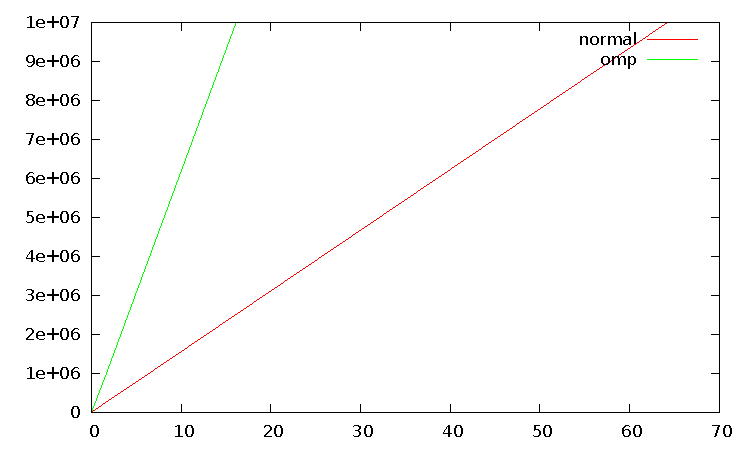
\includegraphics[width=.47\textwidth]{omp} \hspace{2em}
    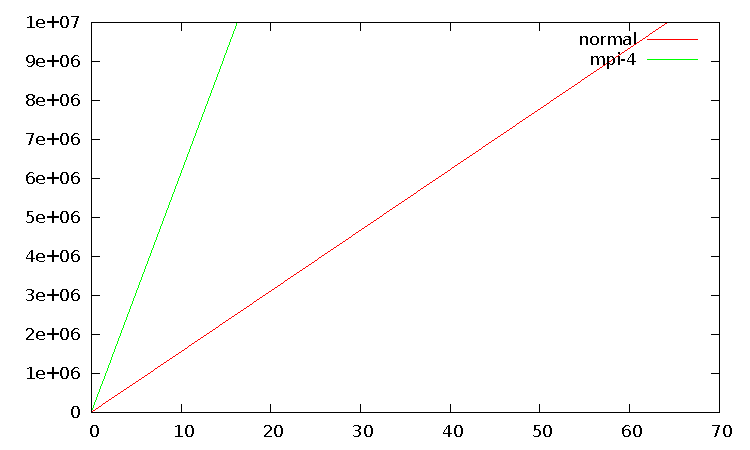
\includegraphics[width=.47\textwidth]{mpi} \\
    \parbox{.47\textwidth}{\center OpenMP} \hspace{2em}
    \parbox{.47\textwidth}{\center MPI}
  \end{figure}
  
  \begin{center}
    \textbf{Division}
  \end{center}
  
  \begin{table}[h!]
    \center
    \begin{tabular}{|C{.05}|*{8}{C{.09}|}} \hline
      count & normal & omp & \multicolumn{2}{c|}{mpi-2} &
        \multicolumn{4}{c|}{mpi-4} \\ \hline
      \( 10^1 \) & \( 2,42 \cdot 10^{-5} \) &
        \( 2,58 \cdot 10^{-5} \) &
        \( 3,57 \cdot 10^{-4} \) & \( 3,82 \cdot 10^{-4} \) &
        \( 4,46 \cdot 10^{-4} \) & \( 6,47 \cdot 10^{-4} \) &
        \( 5,69 \cdot 10^{-4} \) & \( 6,73 \cdot 10^{-4} \) \\ \hline
      \( 10^2 \) & \( 2,40 \cdot 10^{-4} \) &
        \( 2,43 \cdot 10^{-4} \) &
        \( 4,77 \cdot 10^{-4} \) & \( 4,83 \cdot 10^{-4} \) &
        \( 5,41 \cdot 10^{-4} \) & \( 7,00 \cdot 10^{-4} \) &
        \( 9,09 \cdot 10^{-4} \) & \( 8,05 \cdot 10^{-4} \) \\ \hline
      \( 10^4 \) & \( 2,42 \cdot 10^{-2} \) &
        \( 2,43 \cdot 10^{-2} \) &
        \( 1,26 \cdot 10^{-2} \) & \( 1,25 \cdot 10^{-2} \) &
        \( 7,10 \cdot 10^{-3} \) & \( 7,20 \cdot 10^{-3} \) &
        \( 7,20 \cdot 10^{-3} \) & \( 7,18 \cdot 10^{-3} \) \\ \hline
      \( 10^6 \) & \( 2,41 \) &
        \( 2,41 \) &
        \( 1,22 \) & \( 1,21 \) &
        \( 6,31 \cdot 10^{-1} \) & \( 6,33 \cdot 10^{-1} \) &
        \( 6,34 \cdot 10^{-1} \) & \( 6,29 \cdot 10^{-1} \) \\ \hline
      \( 10^7 \) & \( 24,10 \) &
        \( 24,10 \) &
        \( 12,18 \) & \( 12,12 \) &
        \( 6,30 \) & \( 6,26 \) & \( 6,29 \) & \( 6,31 \) \\ \hline
    \end{tabular}
  \end{table}
  
  \begin{center}
    \textbf{Super Functions}
  \end{center}
  
  \begin{table}[h!]
    \center
    \begin{tabular}{|C{.05}|*{8}{C{.09}|}} \hline
      count & normal & omp & \multicolumn{2}{c|}{mpi-2} &
        \multicolumn{4}{c|}{mpi-4} \\ \hline
      \( 10^1 \) & \( 2,60 \cdot 10^{-3} \) &
        \( 2,60 \cdot 10^{-3} \) &
        \( 1,61 \cdot 10^{-3} \) & \( 1,67 \cdot 10^{-3} \) &
        \( 1,20 \cdot 10^{-3} \) & \( 1,40 \cdot 10^{-3} \) &
        \( 1,08 \cdot 10^{-3} \) & \( 1,31 \cdot 10^{-3} \) \\ \hline
      \( 10^2 \) & \( 2,60 \cdot 10^{-2} \) &
        \( 2,60 \cdot 10^{-2} \) &
        \( 1,34 \cdot 10^{-2} \) & \( 1,34 \cdot 10^{-2} \) &
        \( 6,88 \cdot 10^{-3} \) & \( 7,14 \cdot 10^{-3} \) &
        \( 6,99 \cdot 10^{-3} \) & \( 7,07 \cdot 10^{-3} \) \\ \hline
      \( 10^4 \) & \( 2,60 \) &
        \( 2,60 \) &
        \( 1,30 \) & \( 1,30 \) &
        \( 6,54 \cdot 10^{-1} \) & \( 6,54 \cdot 10^{-1} \) &
        \( 6,54 \cdot 10^{-1} \) & \( 6,54 \cdot 10^{-1} \) \\ \hline
      \( 10^6 \) & \( 263 \) &
        \( 262 \) &
        \( 129 \) & \( 130 \) &
        \( 65,9 \) & \( 65,9 \) & \( 65,9 \) & \( 65,7 \) \\ \hline
    \end{tabular}
  \end{table}
  
  \newpage
  
  \begin{center}
    \textbf{Switch}
  \end{center}
  
  \begin{table}[h!]
    \center
    \begin{tabular}{|C{.05}|*{7}{C{.09}|}} \hline
      count & omp & \multicolumn{2}{c|}{mpi-2} &
        \multicolumn{4}{c|}{mpi-4} \\ \hline
      \( 10^1 \) & \( 5,00 \cdot 10^{-5} \) &
        \( 3,45 \cdot 10^{-4} \) & \( 3,83 \cdot 10^{-4} \) &
        \( 4,69 \cdot 10^{-4} \) & \( 5,71 \cdot 10^{-4} \) &
        \( 6,75 \cdot 10^{-4} \) & \( 6,60 \cdot 10^{-4} \) \\ \hline
      \( 10^2 \) & \( 4,83 \cdot 10^{-4} \) &
        \( 5,67 \cdot 10^{-4} \) & \( 5,69 \cdot 10^{-4} \) &
        \( 7,59 \cdot 10^{-4} \) & \( 5,39 \cdot 10^{-4} \) &
        \( 7,19 \cdot 10^{-4} \) & \( 5,93 \cdot 10^{-4} \) \\ \hline
      \( 10^4 \) & \( 4,83 \cdot 10^{-2} \) &
        \( 2,18 \cdot 10^{-2} \) & \( 2,17 \cdot 10^{-2} \) &
        \( 1,19 \cdot 10^{-2} \) & \( 1,23 \cdot 10^{-2} \) &
        \( 7,20 \cdot 10^{-2} \) & \( 7,18 \cdot 10^{-2} \) \\ \hline
      \( 10^6 \) & \( 7,61 \) &
        \( 3,82 \) & \( 3,82 \) &
        \( 1,94 \) & \( 1,94 \) & \( 1,93 \) & \( 1,93 \) \\ \hline
      \( 10^7 \) & \( 76,20 \) &
        \( 38,20 \) & \( 38,19 \) &
        \( 19,30 \) & \( 19,38 \) & \( 19,29 \) & \( 19,32 \) \\ \hline
    \end{tabular}
  \end{table}
  
  \begin{center}
    \textbf{Sunlight}
  \end{center}
  
  \begin{table}[h!]
    \center
    \begin{tabular}{|*{8}{C{.1}|}} \hline
      count & omp & \multicolumn{2}{c|}{mpi-2} &
        \multicolumn{4}{c|}{mpi-4} \\ \hline
      \multicolumn{8}{|c|}{count\_of\_steps = 1} \\ \hline
      10 & \( 2,05 \cdot 10^{-6} \) &
        \( 6,03 \cdot 10^{-4} \) & \( 6,23 \cdot 10^{-4} \) &
        \( 1,17 \cdot 10^{-3} \) & \( 1,07 \cdot 10^{-3} \) &
        \( 9,13 \cdot 10^{-4} \) & \( 1,15 \cdot 10^{-3} \) \\ \hline
      10000 & \( 3,28 \cdot 10^{-5} \) &
        \( 1,04 \cdot 10^{-3} \) & \( 2,46 \cdot 10^{-3} \) &
        \( 3,94 \cdot 10^{-3} \) & \( 2,41 \cdot 10^{-3} \) &
        \( 3,00 \cdot 10^{-3} \) & \( 4,06 \cdot 10^{-3} \) \\ \hline
      1000000 & \( 8,92 \cdot 10^{-3} \) &
        \( 3,48 \cdot 10^{-2} \) & \( 1,83 \cdot 10^{-1} \) &
        \( 2,27 \cdot 10^{-1} \) & \( 8,04 \cdot 10^{-2} \) &
        \( 2,23 \cdot 10^{-1} \) & \( 2,31 \cdot 10^{-1} \) \\ \hline
      \multicolumn{8}{|c|}{count\_of\_steps = 10} \\ \hline
      10 & \( 2,05 \cdot 10^{-6} \) &
        \( 7,22 \cdot 10^{-4} \) & \( 7,48 \cdot 10^{-4} \) &
        \( 2,17 \cdot 10^{-3} \) & \( 3,72 \cdot 10^{-3} \) &
        \( 3,70 \cdot 10^{-3} \) & \( 2,05 \cdot 10^{-3} \) \\ \hline
      10000 & \( 1,22 \cdot 10^{-4} \) &
        \( 3,76 \cdot 10^{-3} \) & \( 2,27 \cdot 10^{-3} \) &
        \( 3,47 \cdot 10^{-2} \) & \( 3,88 \cdot 10^{-2} \) &
        \( 3,47 \cdot 10^{-2} \) & \( 3,56 \cdot 10^{-2} \) \\ \hline
      1000000 & \( 1,27 \cdot 10^{-2} \) &
        \( 2,92 \cdot 10^{-1} \) & \( 4,38 \cdot 10^{-1} \) &
        \( 8,32 \cdot 10^{-1} \) & \( 8,28 \cdot 10^{-1} \) &
        \( 6,85 \cdot 10^{-1} \) & \( 8,40 \cdot 10^{-1} \) \\ \hline
    \end{tabular}
  \end{table}
  
  \begin{center}
    \textbf{Solid Body}
  \end{center}
  
  \begin{table}[h!]
    \center
    \begin{tabular}{|*{8}{C{.1}|}} \hline
      count (x,~y,~z) & omp & \multicolumn{2}{c|}{mpi-2} &
        \multicolumn{4}{c|}{mpi-4} \\ \hline
      \multicolumn{8}{|c|}{count\_of\_steps = 1} \\ \hline
      5 & \( 2,95 \cdot 10^{-2} \) &
        \( 7,13 \cdot 10^{-4} \) & \( 7,46 \cdot 10^{-4} \) &
        \( 1,42 \cdot 10^{-3} \) & \( 1,35 \cdot 10^{-3} \) &
        \( 9,91 \cdot 10^{-4} \) & \( 1,38 \cdot 10^{-3} \) \\ \hline
      50 & \( 1,23 \cdot 10^{-1} \) &
        \( 5,28 \cdot 10^{-2} \) & \( 5,01 \cdot 10^{-2} \) &
        \( 4,44 \cdot 10^{-2} \) & \( 5,53 \cdot 10^{-2} \) &
        \( 4,40 \cdot 10^{-2} \) & \( 5,23 \cdot 10^{-2} \) \\ \hline
      200 & \( 8,97 \) &
        \( 2,97 \) & \( 2,76 \) &
        \( 2,86 \) & \( 3,03 \) & \( 2,90 \) & \( 2,83 \) \\ \hline
      \multicolumn{8}{|c|}{count\_of\_steps = 10} \\ \hline
      5 & \( 3,12 \cdot 10^{-4} \) &
        \( 1,11 \cdot 10^{-3} \) & \( 1,15 \cdot 10^{-3} \) &
        \( 9,89 \cdot 10^{-3} \) & \( 9,19 \cdot 10^{-3} \) &
        \( 8,66 \cdot 10^{-3} \) & \( 9,80 \cdot 10^{-3} \) \\ \hline
      50 & \( 1,25 \) &
        \( 5,18 \cdot 10^{-1} \) & \( 5,16 \cdot 10^{-1} \) &
        \( 5,33 \cdot 10^{-1} \) & \( 5,33 \cdot 10^{-1} \) &
        \( 5,33 \cdot 10^{-1} \) & \( 5,38 \cdot 10^{-1} \) \\ \hline
      200 & \( 89,70 \) &
        \( 25,98 \) & \( 26,18 \) &
        \( 27,86 \) & \( 27,76 \) & \( 27,82 \) & \( 27,78 \) \\ \hline
    \end{tabular}
  \end{table}
\end{document} \newpage
  \documentclass[pscyr,10pt]{hedlab}
\usepackage[russian]{babel}
\usepackage{graphicx}
\graphicspath{{images/}}
\geometry{margin=1cm}

\labnum{2}
\labname{}
\student{Чечеткин~И.~А.}

% --- листинги ---
\usepackage[usenames,dvipsnames]{color}
\usepackage{listings}
\lstdefinelanguage{newbash}{
  alsoletter={[,],>,\\},
  morekeywords={mpiicc,export,scp,source,which,ssh,cd,cp,ls,exit,mpirun,
    sudo,echo,>>,\\,>,diff,unset,make,traceanalyzer,grep,sort},
  morekeywords={[2]ICCROOT,MPIROOT,MICHOME,I_MPI_FABRICS,I_MPI_MIC,
    I_MPI_MIC_POSTFIX,I_MPI_DEBUG,$ICCROOT,$MPIROOT,$MICHOME,$I_MPI_FABRICS,
    $I_MPI_MIC,$I_MPI_MIC_POSTFIX,$I_MPI_DEBUG,OMP_NUM_THREADS,I_MPI_DOMAIN,
    KMP_AFFINITY,I_MPI_PIN_DOMAIN,VT_LOGFILE_FORMAT},
  morestring=[d]{*}{*},
  moredelim=[s][\bfseries\color{Green}]{[r}{]$},  % user
  moredelim=[s][\bfseries\color{Green}]{robo}{$}, % user
  moredelim=[is][basicstyle]{|>}{<|},             % не выделятся
  moredelim=[is][stringstyle]{\{>}{<\}},          % текстовый вывод
}
\lstset{
  inputencoding=utf8,
  basicstyle=\scriptsize\usefont{T2A}{fcr}{m}{n},
  keywordstyle=\bfseries,
  keywordstyle=[2]{\color{blue}},
  commentstyle=\color{red},
  stringstyle=\color{Violet},
  numbers=left,
  numberstyle=\tiny,
  breakatwhitespace=\false,
  breaklines=\true,
  tabsize=2,
  keepspaces=true,
  language=newbash,
}
% xxx -------- xxx

\begin{document}
  \makeheader
  
  \begin{center}
    \textbf{Задание 0~-- Предустановки}
  \end{center}
  
\begin{lstlisting}
[robo05phi@node31 ~]$ export ICCROOT=/opt/intel/compilers/composerxe
[robo05phi@node31 ~]$ export MPIROOT=/opt/intel/compilers/impi/4.1.1.045
[robo05phi@node31 ~]$ export MPIROOT=/opt/intel/compilers/impi/4.1.3.045
[robo05phi@node31 ~]$ sudo scp $ICCROOT/lib/mic/libiomp5.so mic0:/lib64/
  {>[sudo] password for robo05phi:
  libiomp5.so                                   100% 1067KB   1.0MB/s   00:00<}
[robo05phi@node31 ~]$ sudo scp $ICCROOT/lib/mic/libcilkrts.so.5 mic0:/lib64/
  {>libcilkrts.so.5                               100%  300KB 300.3KB/s   00:00<}
[robo05phi@node31 ~]$ source $ICCROOT/bin/compilervars.sh intel64
[robo05phi@node31 ~]$ source $MPIROOT/intel64/bin/mpivars.sh
[robo05phi@node31 ~]$ which |>icc mpiicc<|
  {>/opt/intel/compilers/composer_xe_2013_sp1.1.106/bin/intel64/icc
  /opt/intel/compilers/impi/4.1.3.045/intel64/bin/mpiicc<}
[robo05phi@node31 ~]$ ssh mic0 hostname
  {>node31-mic0.cluster<}
[robo05phi@node31 ~]$ ssh mic0 |>which mpiicc<|
  {>/bin/mpiicc<}
[robo05phi@node31 ~]$ export I_MPI_MIC=1
\end{lstlisting}
  
  \begin{center}
    \textbf{Задание 1~-- Основы}
    
    Чистый MPI. Нативная модель
  \end{center}

\begin{lstlisting}
[robo05phi@node31 ~]$ cd Lab1.2_Intel_MPI_Xeon_PHI/source_codes_from_Intel\(R\)/part3/intel_mpi_lab_C/1_Basic/
[robo05phi@node31 1_Basic]$ export MICHOME=/home/$USER/
[robo05phi@node31 1_Basic]$ mpiicc -o test test.c
[robo05phi@node31 1_Basic]$ export I_MPI_FABRICS=shm:tcp
[robo05phi@node31 1_Basic]$ mpirun -n 2 ./test
  {>Hello world: rank 0 of 2 running on node31.cluster
  Hello world: rank 1 of 2 running on node31.cluster<}
[robo05phi@node31 1_Basic]$ mpiicc -mmic -o test.MIC test.c
[robo05phi@node31 1_Basic]$ scp test.MIC mic0:$MICHOME
  {>test.MIC                                      100%   13KB  12.9KB/s   00:00<}
[robo05phi@node31 1_Basic]$ mpirun -wdir $MICHOME -host node31-mic0 -n 2 ./test.MIC
  {>Hello world: rank 0 of 2 running on node31-mic0.cluster
  Hello world: rank 1 of 2 running on node31-mic0.cluster<}
\end{lstlisting}
  
  \begin{center}
    Запуск MPI приложения с хоста с использованием NFS директории
  \end{center}

\begin{lstlisting}
[robo05phi@node31 1_Basic]$ export MICHOME=/var/public/$USER
[robo05phi@node31 1_Basic]$ cp test.MIC $MICHOME
[robo05phi@node31 1_Basic]$ cp test $MICHOME
[robo05phi@node31 1_Basic]$ cd $MICHOME
[robo05phi@node31 robo05phi]$ ls
  {>Lab1.2_Intel_MPI_Xeon_PHI      test.c         test-openmp.MIC  test_run4.txt
  Lab1.2_Intel_MPI_Xeon_PHI.zip  test.MIC       test_run1.txt    test_run5.txt
  machinefile                    test-openmp    test_run2.txt    test_run6.txt
  test                           test-openmp.c  test_run3.txt<}
[robo05phi@node31 robo05phi]$ mpirun -wdir /var/public/$USER -host node31-mic0 -n 2 ./test.MIC
  {>Hello world: rank 0 of 2 running on node31-mic0.cluster
  Hello world: rank 1 of 2 running on node31-mic0.cluster<}
\end{lstlisting}

  \begin{center}
    Запуск MPI приложения непосредственно из окружения файловой системы
      Xeon Phi
  \end{center}

\begin{lstlisting}
[robo05phi@node31 robo05phi]$ scp test.MIC mic0:~
  {>test.MIC                                      100%   13KB  12.9KB/s   00:00<}
[robo05phi@node31 robo05phi]$ ssh mic0
robo05phi@node31-mic0:~$ ls
  {>test.MIC<}
robo05phi@node31-mic0:~$ mpirun -host mic0 -perhost 60 -np 120 ./test.MIC
  {>Hello world: rank 0 of 120 running on node31-mic0.cluster
  Hello world: rank 1 of 120 running on node31-mic0.cluster
  Hello world: rank 2 of 120 running on node31-mic0.cluster
  Hello world: rank 3 of 120 running on node31-mic0.cluster
  Hello world: rank 4 of 120 running on node31-mic0.cluster
  Hello world: rank 5 of 120 running on node31-mic0.cluster
  Hello world: rank 6 of 120 running on node31-mic0.cluster
  Hello world: rank 7 of 120 running on node31-mic0.cluster
  Hello world: rank 8 of 120 running on node31-mic0.cluster
  Hello world: rank 9 of 120 running on node31-mic0.cluster
  Hello world: rank 10 of 120 running on node31-mic0.cluster
  Hello world: rank 11 of 120 running on node31-mic0.cluster
  Hello world: rank 12 of 120 running on node31-mic0.cluster
  Hello world: rank 13 of 120 running on node31-mic0.cluster
  Hello world: rank 14 of 120 running on node31-mic0.cluster
  Hello world: rank 15 of 120 running on node31-mic0.cluster
  Hello world: rank 16 of 120 running on node31-mic0.cluster
  Hello world: rank 17 of 120 running on node31-mic0.cluster
  Hello world: rank 18 of 120 running on node31-mic0.cluster
  Hello world: rank 19 of 120 running on node31-mic0.cluster
  Hello world: rank 20 of 120 running on node31-mic0.cluster
  Hello world: rank 21 of 120 running on node31-mic0.cluster
  Hello world: rank 22 of 120 running on node31-mic0.cluster
  Hello world: rank 23 of 120 running on node31-mic0.cluster
  Hello world: rank 24 of 120 running on node31-mic0.cluster
  Hello world: rank 25 of 120 running on node31-mic0.cluster
  Hello world: rank 26 of 120 running on node31-mic0.cluster
  Hello world: rank 27 of 120 running on node31-mic0.cluster
  Hello world: rank 28 of 120 running on node31-mic0.cluster
  Hello world: rank 29 of 120 running on node31-mic0.cluster
  Hello world: rank 30 of 120 running on node31-mic0.cluster
  Hello world: rank 31 of 120 running on node31-mic0.cluster
  Hello world: rank 32 of 120 running on node31-mic0.cluster
  Hello world: rank 33 of 120 running on node31-mic0.cluster
  Hello world: rank 34 of 120 running on node31-mic0.cluster
  Hello world: rank 35 of 120 running on node31-mic0.cluster
  Hello world: rank 36 of 120 running on node31-mic0.cluster
  Hello world: rank 37 of 120 running on node31-mic0.cluster
  Hello world: rank 38 of 120 running on node31-mic0.cluster
  Hello world: rank 39 of 120 running on node31-mic0.cluster
  Hello world: rank 40 of 120 running on node31-mic0.cluster
  Hello world: rank 41 of 120 running on node31-mic0.cluster
  Hello world: rank 42 of 120 running on node31-mic0.cluster
  Hello world: rank 43 of 120 running on node31-mic0.cluster
  Hello world: rank 44 of 120 running on node31-mic0.cluster
  Hello world: rank 45 of 120 running on node31-mic0.cluster
  Hello world: rank 46 of 120 running on node31-mic0.cluster
  Hello world: rank 47 of 120 running on node31-mic0.cluster
  Hello world: rank 48 of 120 running on node31-mic0.cluster
  Hello world: rank 49 of 120 running on node31-mic0.cluster
  Hello world: rank 50 of 120 running on node31-mic0.cluster
  Hello world: rank 51 of 120 running on node31-mic0.cluster
  Hello world: rank 52 of 120 running on node31-mic0.cluster
  Hello world: rank 53 of 120 running on node31-mic0.cluster
  Hello world: rank 54 of 120 running on node31-mic0.cluster
  Hello world: rank 55 of 120 running on node31-mic0.cluster
  Hello world: rank 56 of 120 running on node31-mic0.cluster
  Hello world: rank 57 of 120 running on node31-mic0.cluster
  Hello world: rank 58 of 120 running on node31-mic0.cluster
  Hello world: rank 59 of 120 running on node31-mic0.cluster
  Hello world: rank 60 of 120 running on node31-mic0.cluster
  Hello world: rank 61 of 120 running on node31-mic0.cluster
  Hello world: rank 62 of 120 running on node31-mic0.cluster
  Hello world: rank 63 of 120 running on node31-mic0.cluster
  Hello world: rank 64 of 120 running on node31-mic0.cluster
  Hello world: rank 65 of 120 running on node31-mic0.cluster
  Hello world: rank 66 of 120 running on node31-mic0.cluster
  Hello world: rank 67 of 120 running on node31-mic0.cluster
  Hello world: rank 68 of 120 running on node31-mic0.cluster
  Hello world: rank 69 of 120 running on node31-mic0.cluster
  Hello world: rank 70 of 120 running on node31-mic0.cluster
  Hello world: rank 71 of 120 running on node31-mic0.cluster
  Hello world: rank 72 of 120 running on node31-mic0.cluster
  Hello world: rank 73 of 120 running on node31-mic0.cluster
  Hello world: rank 74 of 120 running on node31-mic0.cluster
  Hello world: rank 75 of 120 running on node31-mic0.cluster
  Hello world: rank 76 of 120 running on node31-mic0.cluster
  Hello world: rank 77 of 120 running on node31-mic0.cluster
  Hello world: rank 78 of 120 running on node31-mic0.cluster
  Hello world: rank 79 of 120 running on node31-mic0.cluster
  Hello world: rank 80 of 120 running on node31-mic0.cluster
  Hello world: rank 81 of 120 running on node31-mic0.cluster
  Hello world: rank 82 of 120 running on node31-mic0.cluster
  Hello world: rank 83 of 120 running on node31-mic0.cluster
  Hello world: rank 84 of 120 running on node31-mic0.cluster
  Hello world: rank 85 of 120 running on node31-mic0.cluster
  Hello world: rank 86 of 120 running on node31-mic0.cluster
  Hello world: rank 87 of 120 running on node31-mic0.cluster
  Hello world: rank 88 of 120 running on node31-mic0.cluster
  Hello world: rank 89 of 120 running on node31-mic0.cluster
  Hello world: rank 90 of 120 running on node31-mic0.cluster
  Hello world: rank 91 of 120 running on node31-mic0.cluster
  Hello world: rank 92 of 120 running on node31-mic0.cluster
  Hello world: rank 93 of 120 running on node31-mic0.cluster
  Hello world: rank 94 of 120 running on node31-mic0.cluster
  Hello world: rank 95 of 120 running on node31-mic0.cluster
  Hello world: rank 96 of 120 running on node31-mic0.cluster
  Hello world: rank 97 of 120 running on node31-mic0.cluster
  Hello world: rank 98 of 120 running on node31-mic0.cluster
  Hello world: rank 99 of 120 running on node31-mic0.cluster
  Hello world: rank 100 of 120 running on node31-mic0.cluster
  Hello world: rank 101 of 120 running on node31-mic0.cluster
  Hello world: rank 102 of 120 running on node31-mic0.cluster
  Hello world: rank 103 of 120 running on node31-mic0.cluster
  Hello world: rank 104 of 120 running on node31-mic0.cluster
  Hello world: rank 105 of 120 running on node31-mic0.cluster
  Hello world: rank 106 of 120 running on node31-mic0.cluster
  Hello world: rank 107 of 120 running on node31-mic0.cluster
  Hello world: rank 108 of 120 running on node31-mic0.cluster
  Hello world: rank 109 of 120 running on node31-mic0.cluster
  Hello world: rank 110 of 120 running on node31-mic0.cluster
  Hello world: rank 111 of 120 running on node31-mic0.cluster
  Hello world: rank 112 of 120 running on node31-mic0.cluster
  Hello world: rank 113 of 120 running on node31-mic0.cluster
  Hello world: rank 114 of 120 running on node31-mic0.cluster
  Hello world: rank 115 of 120 running on node31-mic0.cluster
  Hello world: rank 116 of 120 running on node31-mic0.cluster
  Hello world: rank 117 of 120 running on node31-mic0.cluster
  Hello world: rank 118 of 120 running on node31-mic0.cluster
  Hello world: rank 119 of 120 running on node31-mic0.cluster<}
robo05phi@node31-mic0:~$ exit
  {>logout
  Connection to mic0 closed.<}
[robo05phi@node31 robo05phi]$ ssh mic0
robo05phi@node31-mic0:~$ cd /var/public/$USER/
robo05phi@node31-mic0:/var/public/robo05phi$ ls
  {>Lab1.2_Intel_MPI_Xeon_PHI      test.c
  Lab1.2_Intel_MPI_Xeon_PHI.zip  test_run1.txt
  machinefile                    test_run2.txt
  test                           test_run3.txt
  test-openmp                    test_run4.txt
  test-openmp.MIC                test_run5.txt
  test-openmp.c                  test_run6.txt
  test.MIC<}
robo05phi@node31-mic0:/var/public/robo05phi$ mpirun -host mic0 -perhost 60 -np 120 ./test.MIC
  {>Hello world: rank 0 of 120 running on node31-mic0.cluster
  Hello world: rank 1 of 120 running on node31-mic0.cluster
  Hello world: rank 2 of 120 running on node31-mic0.cluster
  Hello world: rank 3 of 120 running on node31-mic0.cluster
  Hello world: rank 4 of 120 running on node31-mic0.cluster
  Hello world: rank 5 of 120 running on node31-mic0.cluster
  Hello world: rank 6 of 120 running on node31-mic0.cluster
  Hello world: rank 7 of 120 running on node31-mic0.cluster
  Hello world: rank 8 of 120 running on node31-mic0.cluster
  Hello world: rank 9 of 120 running on node31-mic0.cluster
  Hello world: rank 10 of 120 running on node31-mic0.cluster
  Hello world: rank 11 of 120 running on node31-mic0.cluster
  Hello world: rank 12 of 120 running on node31-mic0.cluster
  Hello world: rank 13 of 120 running on node31-mic0.cluster
  Hello world: rank 14 of 120 running on node31-mic0.cluster
  Hello world: rank 15 of 120 running on node31-mic0.cluster
  Hello world: rank 16 of 120 running on node31-mic0.cluster
  Hello world: rank 17 of 120 running on node31-mic0.cluster
  Hello world: rank 18 of 120 running on node31-mic0.cluster
  Hello world: rank 19 of 120 running on node31-mic0.cluster
  Hello world: rank 20 of 120 running on node31-mic0.cluster
  Hello world: rank 21 of 120 running on node31-mic0.cluster
  Hello world: rank 22 of 120 running on node31-mic0.cluster
  Hello world: rank 23 of 120 running on node31-mic0.cluster
  Hello world: rank 24 of 120 running on node31-mic0.cluster
  Hello world: rank 25 of 120 running on node31-mic0.cluster
  Hello world: rank 26 of 120 running on node31-mic0.cluster
  Hello world: rank 27 of 120 running on node31-mic0.cluster
  Hello world: rank 28 of 120 running on node31-mic0.cluster
  Hello world: rank 29 of 120 running on node31-mic0.cluster
  Hello world: rank 30 of 120 running on node31-mic0.cluster
  Hello world: rank 31 of 120 running on node31-mic0.cluster
  Hello world: rank 32 of 120 running on node31-mic0.cluster
  Hello world: rank 33 of 120 running on node31-mic0.cluster
  Hello world: rank 34 of 120 running on node31-mic0.cluster
  Hello world: rank 35 of 120 running on node31-mic0.cluster
  Hello world: rank 36 of 120 running on node31-mic0.cluster
  Hello world: rank 37 of 120 running on node31-mic0.cluster
  Hello world: rank 38 of 120 running on node31-mic0.cluster
  Hello world: rank 39 of 120 running on node31-mic0.cluster
  Hello world: rank 40 of 120 running on node31-mic0.cluster
  Hello world: rank 41 of 120 running on node31-mic0.cluster
  Hello world: rank 42 of 120 running on node31-mic0.cluster
  Hello world: rank 43 of 120 running on node31-mic0.cluster
  Hello world: rank 44 of 120 running on node31-mic0.cluster
  Hello world: rank 45 of 120 running on node31-mic0.cluster
  Hello world: rank 46 of 120 running on node31-mic0.cluster
  Hello world: rank 47 of 120 running on node31-mic0.cluster
  Hello world: rank 48 of 120 running on node31-mic0.cluster
  Hello world: rank 49 of 120 running on node31-mic0.cluster
  Hello world: rank 50 of 120 running on node31-mic0.cluster
  Hello world: rank 51 of 120 running on node31-mic0.cluster
  Hello world: rank 52 of 120 running on node31-mic0.cluster
  Hello world: rank 53 of 120 running on node31-mic0.cluster
  Hello world: rank 54 of 120 running on node31-mic0.cluster
  Hello world: rank 55 of 120 running on node31-mic0.cluster
  Hello world: rank 56 of 120 running on node31-mic0.cluster
  Hello world: rank 57 of 120 running on node31-mic0.cluster
  Hello world: rank 58 of 120 running on node31-mic0.cluster
  Hello world: rank 59 of 120 running on node31-mic0.cluster
  Hello world: rank 60 of 120 running on node31-mic0.cluster
  Hello world: rank 61 of 120 running on node31-mic0.cluster
  Hello world: rank 62 of 120 running on node31-mic0.cluster
  Hello world: rank 63 of 120 running on node31-mic0.cluster
  Hello world: rank 64 of 120 running on node31-mic0.cluster
  Hello world: rank 65 of 120 running on node31-mic0.cluster
  Hello world: rank 66 of 120 running on node31-mic0.cluster
  Hello world: rank 67 of 120 running on node31-mic0.cluster
  Hello world: rank 68 of 120 running on node31-mic0.cluster
  Hello world: rank 69 of 120 running on node31-mic0.cluster
  Hello world: rank 70 of 120 running on node31-mic0.cluster
  Hello world: rank 71 of 120 running on node31-mic0.cluster
  Hello world: rank 72 of 120 running on node31-mic0.cluster
  Hello world: rank 73 of 120 running on node31-mic0.cluster
  Hello world: rank 74 of 120 running on node31-mic0.cluster
  Hello world: rank 75 of 120 running on node31-mic0.cluster
  Hello world: rank 76 of 120 running on node31-mic0.cluster
  Hello world: rank 77 of 120 running on node31-mic0.cluster
  Hello world: rank 78 of 120 running on node31-mic0.cluster
  Hello world: rank 79 of 120 running on node31-mic0.cluster
  Hello world: rank 80 of 120 running on node31-mic0.cluster
  Hello world: rank 81 of 120 running on node31-mic0.cluster
  Hello world: rank 82 of 120 running on node31-mic0.cluster
  Hello world: rank 83 of 120 running on node31-mic0.cluster
  Hello world: rank 84 of 120 running on node31-mic0.cluster
  Hello world: rank 85 of 120 running on node31-mic0.cluster
  Hello world: rank 86 of 120 running on node31-mic0.cluster
  Hello world: rank 87 of 120 running on node31-mic0.cluster
  Hello world: rank 88 of 120 running on node31-mic0.cluster
  Hello world: rank 89 of 120 running on node31-mic0.cluster
  Hello world: rank 90 of 120 running on node31-mic0.cluster
  Hello world: rank 91 of 120 running on node31-mic0.cluster
  Hello world: rank 92 of 120 running on node31-mic0.cluster
  Hello world: rank 93 of 120 running on node31-mic0.cluster
  Hello world: rank 94 of 120 running on node31-mic0.cluster
  Hello world: rank 95 of 120 running on node31-mic0.cluster
  Hello world: rank 96 of 120 running on node31-mic0.cluster
  Hello world: rank 97 of 120 running on node31-mic0.cluster
  Hello world: rank 98 of 120 running on node31-mic0.cluster
  Hello world: rank 99 of 120 running on node31-mic0.cluster
  Hello world: rank 100 of 120 running on node31-mic0.cluster
  Hello world: rank 101 of 120 running on node31-mic0.cluster
  Hello world: rank 102 of 120 running on node31-mic0.cluster
  Hello world: rank 103 of 120 running on node31-mic0.cluster
  Hello world: rank 104 of 120 running on node31-mic0.cluster
  Hello world: rank 105 of 120 running on node31-mic0.cluster
  Hello world: rank 106 of 120 running on node31-mic0.cluster
  Hello world: rank 107 of 120 running on node31-mic0.cluster
  Hello world: rank 108 of 120 running on node31-mic0.cluster
  Hello world: rank 109 of 120 running on node31-mic0.cluster
  Hello world: rank 110 of 120 running on node31-mic0.cluster
  Hello world: rank 111 of 120 running on node31-mic0.cluster
  Hello world: rank 112 of 120 running on node31-mic0.cluster
  Hello world: rank 113 of 120 running on node31-mic0.cluster
  Hello world: rank 114 of 120 running on node31-mic0.cluster
  Hello world: rank 115 of 120 running on node31-mic0.cluster
  Hello world: rank 116 of 120 running on node31-mic0.cluster
  Hello world: rank 117 of 120 running on node31-mic0.cluster
  Hello world: rank 118 of 120 running on node31-mic0.cluster
  Hello world: rank 119 of 120 running on node31-mic0.cluster<}
robo05phi@node31-mic0:/var/public/robo05phi$ exit 
  {>logout
  Connection to mic0 closed.<}
\end{lstlisting}

  \begin{center}
    Запуск тестового MPI приложения с хоста в симметричном режиме на хостовых
      CPU и сопроцессоре Xeon Phi
  \end{center}

\begin{lstlisting}
[robo05phi@node31 robo05phi]$ export MICHOME=/var/public/$USER
[robo05phi@node31 robo05phi]$ cd $MICHOME
[robo05phi@node31 robo05phi]$ ls
  {>Lab1.2_Intel_MPI_Xeon_PHI      test.c         test-openmp.MIC  test_run4.txt
  Lab1.2_Intel_MPI_Xeon_PHI.zip  test.MIC       test_run1.txt    test_run5.txt
  machinefile                    test-openmp    test_run2.txt    test_run6.txt
  test                           test-openmp.c  test_run3.txt<}
[robo05phi@node31 robo05phi]$ mpirun -host node31 -n 2 ./test : -wdir $MICHOME -host mic0 -n 4 ./test.MIC
  {>Hello world: rank 0 of 6 running on node31.cluster
  Hello world: rank 1 of 6 running on node31.cluster
  Hello world: rank 2 of 6 running on node31-mic0.cluster
  Hello world: rank 3 of 6 running on node31-mic0.cluster
  Hello world: rank 4 of 6 running on node31-mic0.cluster
  Hello world: rank 5 of 6 running on node31-mic0.cluster<}
[robo05phi@node31 robo05phi]$ echo node31:2 > machinefile
[robo05phi@node31 robo05phi]$ echo mic0:4 >> machinefile
[robo05phi@node31 robo05phi]$ export I_MPI_MIC_POSTFIX=.MIC
[robo05phi@node31 robo05phi]$ mpirun -machinefile machinefile -n 6 ./test
  {>Hello world: rank 0 of 6 running on node31.cluster
  Hello world: rank 1 of 6 running on node31.cluster
  Hello world: rank 2 of 6 running on node31-mic0.cluster
  Hello world: rank 3 of 6 running on node31-mic0.cluster
  Hello world: rank 4 of 6 running on node31-mic0.cluster
  Hello world: rank 5 of 6 running on node31-mic0.cluster<}
[robo05phi@node31 robo05phi]$ export -n I_MPI_MIC_POSTFIX=.MIC
[robo05phi@node31 robo05phi]$ export I_MPI_DEBUG=4
[robo05phi@node31 robo05phi]$ mpirun -n 2 ./test
  {>[1] MPI startup(): shm and tcp data transfer modes
  [0] MPI startup(): shm and tcp data transfer modes
  [0] MPI startup(): Rank    Pid      Node name       Pin cpu
  [0] MPI startup(): 0       32637    node31.cluster  {0,1,2,3,4,5,6,7,16,17,18,19,20,21,22,23}
  [0] MPI startup(): 1       32638    node31.cluster  {8,9,10,11,12,13,14,15,24,25,26,27,28,29,30,31}
  Hello world: rank 0 of 2 running on node31.cluster
  Hello world: rank 1 of 2 running on node31.cluster<}
[robo05phi@node31 robo05phi]$ mpirun -host mic0 -n 2 ./test.MIC
  {>[0] MPI startup(): shm and tcp data transfer modes
  [1] MPI startup(): shm and tcp data transfer modes
  [0] MPI startup(): Rank    Pid      Node name            Pin cpu
  [0] MPI startup(): 0       16094    node31-mic0.cluster  {1,2,3,4,5,6,7,8,9,10,11,12,13,14,15,16,17,18,
                                                            19,20,21,22,23,24,25,26,27,28,29,30,31,32,33,
                                                            34,35,36,37,38,39,40,41,42,43,44,45,46,47,48,
                                                            49,50,51,52,53,54,55,56,57,58,59,60,61,62,63,
                                                            64,65,66,67,68,69,70,71,72,73,74,75,76,77,78,
                                                            79,80,81,82,83,84,85,86,87,88,89,90,91,92,93,
                                                            94,95,96,97,98,99,100,101,102,103,104,105,
                                                            106,107,108,109,110,111,112,113,114,115,116,
                                                            117,118,119,120}
  [0] MPI startup(): 1       16095    node31-mic0.cluster  {0,121,122,123,124,125,126,127,128,129,130,
                                                            131,132,133,134,135,136,137,138,139,140,141,
                                                            142,143,144,145,146,147,148,149,150,151,152,
                                                            153,154,155,156,157,158,159,160,161,162,163,
                                                            164,165,166,167,168,169,170,171,172,173,174,
                                                            175,176,177,178,179,180,181,182,183,184,185,
                                                            186,187,188,189,190,191,192,193,194,195,196,
                                                            197,198,199,200,201,202,203,204,205,206,207,
                                                            208,209,210,211,212,213,214,215,216,217,218,
                                                            219,220,221,222,223,224,225,226,227,228,229,
                                                            230,231,232,233,234,235,236,237,238,239}
  Hello world: rank 0 of 2 running on node31-mic0.cluster
  Hello world: rank 1 of 2 running on node31-mic0.cluster<}
[robo05phi@node31 robo05phi]$ mpirun -host node31 -n 2 ./test : -host mic0 -n 4 ./test.MIC
  {>[1] MPI startup(): shm and tcp data transfer modes
  [0] MPI startup(): shm and tcp data transfer modes
  [3] MPI startup(): shm and tcp data transfer modes
  [4] MPI startup(): shm and tcp data transfer modes
  [2] MPI startup(): shm and tcp data transfer modes
  [5] MPI startup(): shm and tcp data transfer modes
  [0] MPI startup(): Rank    Pid      Node name            Pin cpu
  [0] MPI startup(): 0       32666    node31.cluster       {0,1,2,3,4,5,6,7,16,17,18,19,20,21,22,23}
  [0] MPI startup(): 1       32667    node31.cluster       {8,9,10,11,12,13,14,15,24,25,26,27,28,29,30,31}
  [0] MPI startup(): 2       16100    node31-mic0.cluster  {1,2,3,4,5,6,7,8,9,10,11,12,13,14,15,16,17,18,
                                                           19,20,21,22,23,24,25,26,27,28,29,30,31,32,33,
                                                           34,35,36,37,38,39,40,41,42,43,44,45,46,47,48,
                                                           49,50,51,52,53,54,55,56,57,58,59,60}
  [0] MPI startup(): 3       16101    node31-mic0.cluster  {61,62,63,64,65,66,67,68,69,70,71,72,73,74,75,
                                                           76,77,78,79,80,81,82,83,84,85,86,87,88,89,90,
                                                           91,92,93,94,95,96,97,98,99,100,101,102,103,104,
                                                           105,106,107,108,109,110,111,112,113,114,115,116,
                                                           117,118,119,120}
  [0] MPI startup(): 4       16102    node31-mic0.cluster  {121,122,123,124,125,126,127,128,129,130,
                                                           131,132,133,134,135,136,137,138,139,140,141,142,
                                                           143,144,145,146,147,148,149,150,151,152,153,154,
                                                           155,156,157,158,159,160,161,162,163,164,165,166,
                                                           167,168,169,170,171,172,173,174,175,176,177,178,
                                                           179,180}
  [0] MPI startup(): 5       16103    node31-mic0.cluster  {0,181,182,183,184,185,186,187,188,189,
                                                           190,191,192,193,194,195,196,197,198,199,200,201,
                                                           202,203,204,205,206,207,208,209,210,211,212,213,
                                                           214,215,216,217,218,219,220,221,222,223,224,225,
                                                           226,227,228,229,230,231,232,233,234,235,236,237,
                                                           238,239}
  Hello world: rank 0 of 6 running on node31.cluster
  Hello world: rank 1 of 6 running on node31.cluster
  Hello world: rank 2 of 6 running on node31-mic0.cluster
  Hello world: rank 3 of 6 running on node31-mic0.cluster
  Hello world: rank 4 of 6 running on node31-mic0.cluster
  Hello world: rank 5 of 6 running on node31-mic0.cluster<}
[robo05phi@node31 robo05phi]$ mpirun -env I_MPI_PIN_DOMAIN auto -n 2 ./test
  {>[1] MPI startup(): shm and tcp data transfer modes
  [0] MPI startup(): shm and tcp data transfer modes
  [0] MPI startup(): Rank    Pid      Node name       Pin cpu
  [0] MPI startup(): 0       32727    node31.cluster  {0,1,2,3,4,5,6,7,16,17,18,19,20,21,22,23}
  [0] MPI startup(): 1       32728    node31.cluster  {8,9,10,11,12,13,14,15,24,25,26,27,28,29,30,31}
  Hello world: rank 0 of 2 running on node31.cluster
  Hello world: rank 1 of 2 running on node31.cluster<}
[robo05phi@node31 robo05phi]$ mpirun -env I_MPI_PIN_DOMAIN auto -host mic0 -n 2 ./test.MIC
  {>[0] MPI startup(): shm and tcp data transfer modes
  [1] MPI startup(): shm and tcp data transfer modes
  [0] MPI startup(): Rank    Pid      Node name            Pin cpu
  [0] MPI startup(): 0       16121    node31-mic0.cluster  {1,2,3,4,5,6,7,8,9,10,11,12,13,14,15,16,17,18,
                                                         19,20,21,22,23,24,25,26,27,28,29,30,31,32,33,
                                                         34,35,36,37,38,39,40,41,42,43,44,45,46,47,48,
                                                         49,50,51,52,53,54,55,56,57,58,59,60,61,62,63,
                                                         64,65,66,67,68,69,70,71,72,73,74,75,76,77,78,
                                                         79,80,81,82,83,84,85,86,87,88,89,90,91,92,93,
                                                         94,95,96,97,98,99,100,101,102,103,104,105,
                                                         106,107,108,109,110,111,112,113,114,115,116,
                                                         117,118,119,120}
  [0] MPI startup(): 1       16122    node31-mic0.cluster  {0,121,122,123,124,125,126,127,128,129,130,
                                                         131,132,133,134,135,136,137,138,139,140,141,142,
                                                         143,144,145,146,147,148,149,150,151,152,153,154,
                                                         155,156,157,158,159,160,161,162,163,164,165,166,
                                                         167,168,169,170,171,172,173,174,175,176,177,178,
                                                         179,180,181,182,183,184,185,186,187,188,189,190,
                                                         191,192,193,194,195,196,197,198,199,200,201,202,
                                                         203,204,205,206,207,208,209,210,211,212,213,214,
                                                         215,216,217,218,219,220,221,222,223,224,225,226,
                                                         227,228,229,230,231,232,233,234,235,236,237,238,
                                                         239}
  Hello world: rank 0 of 2 running on node31-mic0.cluster
  Hello world: rank 1 of 2 running on node31-mic0.cluster<}
[robo05phi@node31 robo05phi]$ mpirun -env I_MPI_PIN_DOMAIN 4 -host node31 -n 2 ./test : -env I_MPI_PIN_DOMAIN 12 \
-host mic0 -n 4 ./test.MIC
  {>[0] MPI startup(): shm and tcp data transfer modes
[1] MPI startup(): shm and tcp data transfer modes
  [2] MPI startup(): shm and tcp data transfer modes
  [3] MPI startup(): shm and tcp data transfer modes
  [4] MPI startup(): shm and tcp data transfer modes
  [5] MPI startup(): shm and tcp data transfer modes
  [0] MPI startup(): Rank    Pid      Node name            Pin cpu
  [0] MPI startup(): 0       315      node31.cluster       {0,1,16,17}
  [0] MPI startup(): 1       316      node31.cluster       {2,3,18,19}
  [0] MPI startup(): 2       16130    node31-mic0.cluster  {1,2,3,4,5,6,7,8,9,10,11,12}
  [0] MPI startup(): 3       16131    node31-mic0.cluster  {13,14,15,16,17,18,19,20,21,22,23,24}
  [0] MPI startup(): 4       16132    node31-mic0.cluster  {25,26,27,28,29,30,31,32,33,34,35,36}
  [0] MPI startup(): 5       16133    node31-mic0.cluster  {37,38,39,40,41,42,43,44,45,46,47,48}
  Hello world: rank 0 of 6 running on node31.cluster
  Hello world: rank 1 of 6 running on node31.cluster
  Hello world: rank 2 of 6 running on node31-mic0.cluster
  Hello world: rank 3 of 6 running on node31-mic0.cluster
  Hello world: rank 4 of 6 running on node31-mic0.cluster
  Hello world: rank 5 of 6 running on node31-mic0.cluster<}
\end{lstlisting}

  \begin{center}
    Знакомство с гибридными MPI/OpenMPI приложениями для сопроцессора
  \end{center}

\begin{lstlisting}
[robo05phi@node31 robo05phi]$ diff test.c test-openmp.c
  {>22a23,25
  > #ifdef _OPENMP
  > #include <omp.h>
  > #endif
  36a40,46
  > #ifdef _OPENMP
  > #pragma omp parallel
  >     {
  > 	printf ("Hello world: rank %d of %d running on %s: thread %d\n", rank, size, name, omp_get_thread_num());
  >     }
  > #endif
  > <}
[robo05phi@node31 robo05phi]$ mpiicc -openmp -o test-openmp test-openmp.c
[robo05phi@node31 robo05phi]$ mpiicc -openmp -mmic -o test-openmp.MIC test-openmp.c
[robo05phi@node31 robo05phi]$ unset I_MPI_DEBUG
[robo05phi@node31 robo05phi]$ mpirun -n 2 ./test-openmp
  {>Hello world: rank 0 of 2 running on node31.cluster: thread 0
  Hello world: rank 0 of 2 running on node31.cluster: thread 11
  Hello world: rank 0 of 2 running on node31.cluster: thread 1
  Hello world: rank 0 of 2 running on node31.cluster: thread 9
  Hello world: rank 0 of 2 running on node31.cluster: thread 13
  Hello world: rank 0 of 2 running on node31.cluster: thread 3
  Hello world: rank 0 of 2 running on node31.cluster: thread 12
  Hello world: rank 0 of 2 running on node31.cluster: thread 2
  Hello world: rank 0 of 2 running on node31.cluster: thread 4
  Hello world: rank 0 of 2 running on node31.cluster: thread 6
  Hello world: rank 0 of 2 running on node31.cluster: thread 10
  Hello world: rank 1 of 2 running on node31.cluster: thread 0
  Hello world: rank 1 of 2 running on node31.cluster: thread 9
  Hello world: rank 1 of 2 running on node31.cluster: thread 14
  Hello world: rank 1 of 2 running on node31.cluster: thread 4
  Hello world: rank 1 of 2 running on node31.cluster: thread 6
  Hello world: rank 1 of 2 running on node31.cluster: thread 3
  Hello world: rank 1 of 2 running on node31.cluster: thread 2
  Hello world: rank 1 of 2 running on node31.cluster: thread 8
  Hello world: rank 1 of 2 running on node31.cluster: thread 10
  Hello world: rank 1 of 2 running on node31.cluster: thread 1
  Hello world: rank 1 of 2 running on node31.cluster: thread 15
  Hello world: rank 1 of 2 running on node31.cluster: thread 5
  Hello world: rank 0 of 2 running on node31.cluster: thread 7
  Hello world: rank 0 of 2 running on node31.cluster: thread 5
  Hello world: rank 0 of 2 running on node31.cluster: thread 14
  Hello world: rank 0 of 2 running on node31.cluster: thread 8
  Hello world: rank 1 of 2 running on node31.cluster: thread 11
  Hello world: rank 1 of 2 running on node31.cluster: thread 12
  Hello world: rank 1 of 2 running on node31.cluster: thread 7
  Hello world: rank 1 of 2 running on node31.cluster: thread 13
  Hello world: rank 0 of 2 running on node31.cluster: thread 15
  Hello world: rank 0 of 2 running on node31.cluster
  Hello world: rank 1 of 2 running on node31.cluster<}
[robo05phi@node31 robo05phi]$ mpirun -host mic0 -n 2 ./test-openmp.MIC
  {>Hello world: rank 1 of 2 running on node31-mic0.cluster: thread 0
  Hello world: rank 1 of 2 running on node31-mic0.cluster: thread 66
  Hello world: rank 1 of 2 running on node31-mic0.cluster: thread 77
  Hello world: rank 1 of 2 running on node31-mic0.cluster: thread 108
  Hello world: rank 1 of 2 running on node31-mic0.cluster: thread 98
  Hello world: rank 1 of 2 running on node31-mic0.cluster: thread 60
  Hello world: rank 1 of 2 running on node31-mic0.cluster: thread 35
  Hello world: rank 1 of 2 running on node31-mic0.cluster: thread 61
  Hello world: rank 1 of 2 running on node31-mic0.cluster: thread 23
  Hello world: rank 1 of 2 running on node31-mic0.cluster: thread 15
  Hello world: rank 1 of 2 running on node31-mic0.cluster: thread 30
  Hello world: rank 1 of 2 running on node31-mic0.cluster: thread 78
  Hello world: rank 1 of 2 running on node31-mic0.cluster: thread 16
  Hello world: rank 1 of 2 running on node31-mic0.cluster: thread 37
  Hello world: rank 1 of 2 running on node31-mic0.cluster: thread 55
  Hello world: rank 1 of 2 running on node31-mic0.cluster: thread 56
  Hello world: rank 1 of 2 running on node31-mic0.cluster: thread 49
  Hello world: rank 1 of 2 running on node31-mic0.cluster: thread 85
  Hello world: rank 1 of 2 running on node31-mic0.cluster: thread 68
  Hello world: rank 1 of 2 running on node31-mic0.cluster: thread 95
  Hello world: rank 1 of 2 running on node31-mic0.cluster: thread 53
  Hello world: rank 1 of 2 running on node31-mic0.cluster: thread 83
  Hello world: rank 1 of 2 running on node31-mic0.cluster: thread 4
  Hello world: rank 1 of 2 running on node31-mic0.cluster: thread 80
  Hello world: rank 1 of 2 running on node31-mic0.cluster: thread 12
  Hello world: rank 1 of 2 running on node31-mic0.cluster: thread 9
  Hello world: rank 1 of 2 running on node31-mic0.cluster: thread 10
  Hello world: rank 1 of 2 running on node31-mic0.cluster: thread 6
  Hello world: rank 1 of 2 running on node31-mic0.cluster: thread 96
  Hello world: rank 1 of 2 running on node31-mic0.cluster: thread 18
  Hello world: rank 1 of 2 running on node31-mic0.cluster: thread 19
  Hello world: rank 1 of 2 running on node31-mic0.cluster: thread 3
  Hello world: rank 1 of 2 running on node31-mic0.cluster: thread 114
  Hello world: rank 1 of 2 running on node31-mic0.cluster: thread 25
  Hello world: rank 1 of 2 running on node31-mic0.cluster: thread 21
  Hello world: rank 1 of 2 running on node31-mic0.cluster: thread 26
  Hello world: rank 1 of 2 running on node31-mic0.cluster: thread 22
  Hello world: rank 1 of 2 running on node31-mic0.cluster: thread 112
  Hello world: rank 1 of 2 running on node31-mic0.cluster: thread 82
  Hello world: rank 1 of 2 running on node31-mic0.cluster: thread 20
  Hello world: rank 1 of 2 running on node31-mic0.cluster: thread 76
  Hello world: rank 1 of 2 running on node31-mic0.cluster: thread 100
  Hello world: rank 1 of 2 running on node31-mic0.cluster: thread 74
  Hello world: rank 1 of 2 running on node31-mic0.cluster: thread 11
  Hello world: rank 1 of 2 running on node31-mic0.cluster: thread 7
  Hello world: rank 1 of 2 running on node31-mic0.cluster: thread 67
  Hello world: rank 1 of 2 running on node31-mic0.cluster: thread 104
  Hello world: rank 1 of 2 running on node31-mic0.cluster: thread 28
  Hello world: rank 1 of 2 running on node31-mic0.cluster: thread 116
  Hello world: rank 1 of 2 running on node31-mic0.cluster: thread 86
  Hello world: rank 1 of 2 running on node31-mic0.cluster: thread 118
  Hello world: rank 1 of 2 running on node31-mic0.cluster: thread 113
  Hello world: rank 1 of 2 running on node31-mic0.cluster: thread 99
  Hello world: rank 1 of 2 running on node31-mic0.cluster: thread 106
  Hello world: rank 1 of 2 running on node31-mic0.cluster: thread 32
  Hello world: rank 1 of 2 running on node31-mic0.cluster: thread 102
  Hello world: rank 1 of 2 running on node31-mic0.cluster: thread 92
  Hello world: rank 1 of 2 running on node31-mic0.cluster: thread 117
  Hello world: rank 1 of 2 running on node31-mic0.cluster: thread 87
  Hello world: rank 1 of 2 running on node31-mic0.cluster: thread 101
  Hello world: rank 1 of 2 running on node31-mic0.cluster: thread 89
  Hello world: rank 1 of 2 running on node31-mic0.cluster: thread 119
  Hello world: rank 1 of 2 running on node31-mic0.cluster: thread 29
  Hello world: rank 0 of 2 running on node31-mic0.cluster: thread 0
  Hello world: rank 0 of 2 running on node31-mic0.cluster: thread 65
  Hello world: rank 0 of 2 running on node31-mic0.cluster: thread 50
  Hello world: rank 0 of 2 running on node31-mic0.cluster: thread 8
  Hello world: rank 0 of 2 running on node31-mic0.cluster: thread 98
  Hello world: rank 0 of 2 running on node31-mic0.cluster: thread 43
  Hello world: rank 1 of 2 running on node31-mic0.cluster: thread 107
  Hello world: rank 1 of 2 running on node31-mic0.cluster: thread 79
  Hello world: rank 1 of 2 running on node31-mic0.cluster: thread 33
  Hello world: rank 1 of 2 running on node31-mic0.cluster: thread 36
  Hello world: rank 1 of 2 running on node31-mic0.cluster: thread 111
  Hello world: rank 1 of 2 running on node31-mic0.cluster: thread 93
  Hello world: rank 1 of 2 running on node31-mic0.cluster: thread 40
  Hello world: rank 1 of 2 running on node31-mic0.cluster: thread 41
  Hello world: rank 1 of 2 running on node31-mic0.cluster: thread 54
  Hello world: rank 1 of 2 running on node31-mic0.cluster: thread 38
  Hello world: rank 0 of 2 running on node31-mic0.cluster: thread 108
  Hello world: rank 0 of 2 running on node31-mic0.cluster: thread 95
  Hello world: rank 0 of 2 running on node31-mic0.cluster: thread 109
  Hello world: rank 0 of 2 running on node31-mic0.cluster: thread 111
  Hello world: rank 0 of 2 running on node31-mic0.cluster: thread 112
  Hello world: rank 0 of 2 running on node31-mic0.cluster: thread 88
  Hello world: rank 0 of 2 running on node31-mic0.cluster: thread 44
  Hello world: rank 0 of 2 running on node31-mic0.cluster: thread 96
  Hello world: rank 0 of 2 running on node31-mic0.cluster: thread 26
  Hello world: rank 0 of 2 running on node31-mic0.cluster: thread 85
  Hello world: rank 0 of 2 running on node31-mic0.cluster: thread 77
  Hello world: rank 0 of 2 running on node31-mic0.cluster: thread 45
  Hello world: rank 0 of 2 running on node31-mic0.cluster: thread 117
  Hello world: rank 0 of 2 running on node31-mic0.cluster: thread 99
  Hello world: rank 0 of 2 running on node31-mic0.cluster: thread 47
  Hello world: rank 0 of 2 running on node31-mic0.cluster: thread 110
  Hello world: rank 1 of 2 running on node31-mic0.cluster: thread 31
  Hello world: rank 1 of 2 running on node31-mic0.cluster: thread 91
  Hello world: rank 1 of 2 running on node31-mic0.cluster: thread 90
  Hello world: rank 1 of 2 running on node31-mic0.cluster: thread 48
  Hello world: rank 1 of 2 running on node31-mic0.cluster: thread 34
  Hello world: rank 1 of 2 running on node31-mic0.cluster: thread 94
  Hello world: rank 1 of 2 running on node31-mic0.cluster: thread 42
  Hello world: rank 1 of 2 running on node31-mic0.cluster: thread 44
  Hello world: rank 1 of 2 running on node31-mic0.cluster: thread 103
  Hello world: rank 1 of 2 running on node31-mic0.cluster: thread 39
  Hello world: rank 0 of 2 running on node31-mic0.cluster: thread 59
  Hello world: rank 0 of 2 running on node31-mic0.cluster: thread 105
  Hello world: rank 0 of 2 running on node31-mic0.cluster: thread 80
  Hello world: rank 0 of 2 running on node31-mic0.cluster: thread 106
  Hello world: rank 0 of 2 running on node31-mic0.cluster: thread 63
  Hello world: rank 0 of 2 running on node31-mic0.cluster: thread 2
  Hello world: rank 0 of 2 running on node31-mic0.cluster: thread 18
  Hello world: rank 0 of 2 running on node31-mic0.cluster: thread 10
  Hello world: rank 0 of 2 running on node31-mic0.cluster: thread 3
  Hello world: rank 0 of 2 running on node31-mic0.cluster: thread 115
  Hello world: rank 0 of 2 running on node31-mic0.cluster: thread 69
  Hello world: rank 0 of 2 running on node31-mic0.cluster: thread 16
  Hello world: rank 0 of 2 running on node31-mic0.cluster: thread 4
  Hello world: rank 0 of 2 running on node31-mic0.cluster: thread 64
  Hello world: rank 0 of 2 running on node31-mic0.cluster: thread 13
  Hello world: rank 0 of 2 running on node31-mic0.cluster: thread 35
  Hello world: rank 0 of 2 running on node31-mic0.cluster: thread 72
  Hello world: rank 0 of 2 running on node31-mic0.cluster: thread 66
  Hello world: rank 0 of 2 running on node31-mic0.cluster: thread 11
  Hello world: rank 0 of 2 running on node31-mic0.cluster: thread 48
  Hello world: rank 0 of 2 running on node31-mic0.cluster: thread 70
  Hello world: rank 0 of 2 running on node31-mic0.cluster: thread 40
  Hello world: rank 0 of 2 running on node31-mic0.cluster: thread 22
  Hello world: rank 0 of 2 running on node31-mic0.cluster: thread 82
  Hello world: rank 0 of 2 running on node31-mic0.cluster: thread 33
  Hello world: rank 0 of 2 running on node31-mic0.cluster: thread 114
  Hello world: rank 0 of 2 running on node31-mic0.cluster: thread 34
  Hello world: rank 0 of 2 running on node31-mic0.cluster: thread 68
  Hello world: rank 0 of 2 running on node31-mic0.cluster: thread 81
  Hello world: rank 1 of 2 running on node31-mic0.cluster: thread 46
  Hello world: rank 1 of 2 running on node31-mic0.cluster: thread 50
  Hello world: rank 1 of 2 running on node31-mic0.cluster: thread 110
  Hello world: rank 1 of 2 running on node31-mic0.cluster: thread 58
  Hello world: rank 1 of 2 running on node31-mic0.cluster: thread 47
  Hello world: rank 1 of 2 running on node31-mic0.cluster: thread 51
  Hello world: rank 1 of 2 running on node31-mic0.cluster: thread 45
  Hello world: rank 1 of 2 running on node31-mic0.cluster: thread 97
  Hello world: rank 1 of 2 running on node31-mic0.cluster: thread 52
  Hello world: rank 1 of 2 running on node31-mic0.cluster: thread 43
  Hello world: rank 1 of 2 running on node31-mic0.cluster: thread 62
  Hello world: rank 1 of 2 running on node31-mic0.cluster: thread 88
  Hello world: rank 1 of 2 running on node31-mic0.cluster: thread 63
  Hello world: rank 1 of 2 running on node31-mic0.cluster: thread 59
  Hello world: rank 1 of 2 running on node31-mic0.cluster: thread 2
  Hello world: rank 1 of 2 running on node31-mic0.cluster: thread 75
  Hello world: rank 1 of 2 running on node31-mic0.cluster: thread 105
  Hello world: rank 1 of 2 running on node31-mic0.cluster: thread 109
  Hello world: rank 1 of 2 running on node31-mic0.cluster: thread 8
  Hello world: rank 1 of 2 running on node31-mic0.cluster: thread 57
  Hello world: rank 1 of 2 running on node31-mic0.cluster: thread 64
  Hello world: rank 1 of 2 running on node31-mic0.cluster: thread 17
  Hello world: rank 1 of 2 running on node31-mic0.cluster: thread 65
  Hello world: rank 1 of 2 running on node31-mic0.cluster: thread 5
  Hello world: rank 1 of 2 running on node31-mic0.cluster: thread 72
  Hello world: rank 1 of 2 running on node31-mic0.cluster: thread 69
  Hello world: rank 1 of 2 running on node31-mic0.cluster: thread 70
  Hello world: rank 1 of 2 running on node31-mic0.cluster: thread 24
  Hello world: rank 1 of 2 running on node31-mic0.cluster: thread 81
  Hello world: rank 1 of 2 running on node31-mic0.cluster: thread 115
  Hello world: rank 1 of 2 running on node31-mic0.cluster: thread 13
  Hello world: rank 1 of 2 running on node31-mic0.cluster: thread 1
  Hello world: rank 1 of 2 running on node31-mic0.cluster: thread 73
  Hello world: rank 1 of 2 running on node31-mic0.cluster: thread 84
  Hello world: rank 1 of 2 running on node31-mic0.cluster: thread 14
  Hello world: rank 1 of 2 running on node31-mic0.cluster: thread 71
  Hello world: rank 1 of 2 running on node31-mic0.cluster: thread 27
  Hello world: rank 0 of 2 running on node31-mic0.cluster: thread 21
  Hello world: rank 0 of 2 running on node31-mic0.cluster: thread 5
  Hello world: rank 0 of 2 running on node31-mic0.cluster: thread 76
  Hello world: rank 0 of 2 running on node31-mic0.cluster: thread 7
  Hello world: rank 0 of 2 running on node31-mic0.cluster: thread 67
  Hello world: rank 0 of 2 running on node31-mic0.cluster: thread 14
  Hello world: rank 0 of 2 running on node31-mic0.cluster: thread 118
  Hello world: rank 0 of 2 running on node31-mic0.cluster: thread 42
  Hello world: rank 0 of 2 running on node31-mic0.cluster: thread 71
  Hello world: rank 0 of 2 running on node31-mic0.cluster: thread 24
  Hello world: rank 0 of 2 running on node31-mic0.cluster: thread 52
  Hello world: rank 0 of 2 running on node31-mic0.cluster: thread 113
  Hello world: rank 0 of 2 running on node31-mic0.cluster: thread 89
  Hello world: rank 0 of 2 running on node31-mic0.cluster: thread 29
  Hello world: rank 0 of 2 running on node31-mic0.cluster: thread 116
  Hello world: rank 0 of 2 running on node31-mic0.cluster: thread 119
  Hello world: rank 0 of 2 running on node31-mic0.cluster: thread 83
  Hello world: rank 0 of 2 running on node31-mic0.cluster: thread 38
  Hello world: rank 0 of 2 running on node31-mic0.cluster: thread 25
  Hello world: rank 0 of 2 running on node31-mic0.cluster: thread 56
  Hello world: rank 0 of 2 running on node31-mic0.cluster: thread 92
  Hello world: rank 0 of 2 running on node31-mic0.cluster: thread 23
  Hello world: rank 0 of 2 running on node31-mic0.cluster: thread 75
  Hello world: rank 0 of 2 running on node31-mic0.cluster: thread 15
  Hello world: rank 0 of 2 running on node31-mic0.cluster: thread 30
  Hello world: rank 0 of 2 running on node31-mic0.cluster: thread 90
  Hello world: rank 0 of 2 running on node31-mic0.cluster: thread 100
  Hello world: rank 0 of 2 running on node31-mic0.cluster: thread 39
  Hello world: rank 0 of 2 running on node31-mic0.cluster: thread 46
  Hello world: rank 0 of 2 running on node31-mic0.cluster: thread 78
  Hello world: rank 0 of 2 running on node31-mic0.cluster: thread 87
  Hello world: rank 0 of 2 running on node31-mic0.cluster: thread 54
  Hello world: rank 0 of 2 running on node31-mic0.cluster: thread 51
  Hello world: rank 0 of 2 running on node31-mic0.cluster: thread 58
  Hello world: rank 0 of 2 running on node31-mic0.cluster: thread 97
  Hello world: rank 0 of 2 running on node31-mic0.cluster: thread 53
  Hello world: rank 0 of 2 running on node31-mic0.cluster: thread 93
  Hello world: rank 0 of 2 running on node31-mic0.cluster: thread 60
  Hello world: rank 0 of 2 running on node31-mic0.cluster: thread 104
  Hello world: rank 0 of 2 running on node31-mic0.cluster: thread 94
  Hello world: rank 0 of 2 running on node31-mic0.cluster: thread 102
  Hello world: rank 0 of 2 running on node31-mic0.cluster: thread 79
  Hello world: rank 0 of 2 running on node31-mic0.cluster: thread 55
  Hello world: rank 0 of 2 running on node31-mic0.cluster: thread 31
  Hello world: rank 0 of 2 running on node31-mic0.cluster: thread 91
  Hello world: rank 0 of 2 running on node31-mic0.cluster: thread 62
  Hello world: rank 0 of 2 running on node31-mic0.cluster: thread 103
  Hello world: rank 0 of 2 running on node31-mic0.cluster: thread 19
  Hello world: rank 0 of 2 running on node31-mic0.cluster: thread 49
  Hello world: rank 0 of 2 running on node31-mic0.cluster: thread 61
  Hello world: rank 0 of 2 running on node31-mic0.cluster: thread 107
  Hello world: rank 0 of 2 running on node31-mic0.cluster: thread 28
  Hello world: rank 0 of 2 running on node31-mic0.cluster: thread 74
  Hello world: rank 0 of 2 running on node31-mic0.cluster: thread 1
  Hello world: rank 0 of 2 running on node31-mic0.cluster: thread 32
  Hello world: rank 0 of 2 running on node31-mic0.cluster: thread 17
  Hello world: rank 0 of 2 running on node31-mic0.cluster: thread 27
  Hello world: rank 0 of 2 running on node31-mic0.cluster: thread 101
  Hello world: rank 0 of 2 running on node31-mic0.cluster: thread 20
  Hello world: rank 0 of 2 running on node31-mic0.cluster: thread 57
  Hello world: rank 0 of 2 running on node31-mic0.cluster: thread 12
  Hello world: rank 0 of 2 running on node31-mic0.cluster: thread 86
  Hello world: rank 0 of 2 running on node31-mic0.cluster: thread 36
  Hello world: rank 0 of 2 running on node31-mic0.cluster: thread 73
  Hello world: rank 0 of 2 running on node31-mic0.cluster: thread 84
  Hello world: rank 0 of 2 running on node31-mic0.cluster: thread 37
  Hello world: rank 0 of 2 running on node31-mic0.cluster: thread 41
  Hello world: rank 0 of 2 running on node31-mic0.cluster: thread 6
  Hello world: rank 0 of 2 running on node31-mic0.cluster: thread 9
  Hello world: rank 0 of 2 running on node31-mic0.cluster
  Hello world: rank 1 of 2 running on node31-mic0.cluster<}
[robo05phi@node31 robo05phi]$ mpirun -host node31 -n 2 ./test-openmp : -host mic0 -n 4 ./test-openmp.MIC
  {>Hello world: rank 0 of 6 running on node31.cluster: thread 0
  Hello world: rank 0 of 6 running on node31.cluster: thread 14
  Hello world: rank 0 of 6 running on node31.cluster: thread 2
  Hello world: rank 0 of 6 running on node31.cluster: thread 4
  Hello world: rank 0 of 6 running on node31.cluster: thread 7
  Hello world: rank 0 of 6 running on node31.cluster: thread 6
  Hello world: rank 0 of 6 running on node31.cluster: thread 3
  Hello world: rank 0 of 6 running on node31.cluster: thread 1
  Hello world: rank 0 of 6 running on node31.cluster: thread 10
  Hello world: rank 0 of 6 running on node31.cluster: thread 15
  Hello world: rank 0 of 6 running on node31.cluster: thread 8
  Hello world: rank 0 of 6 running on node31.cluster: thread 13
  Hello world: rank 1 of 6 running on node31.cluster: thread 0
  Hello world: rank 1 of 6 running on node31.cluster: thread 8
  Hello world: rank 1 of 6 running on node31.cluster: thread 15
  Hello world: rank 1 of 6 running on node31.cluster: thread 12
  Hello world: rank 1 of 6 running on node31.cluster: thread 1
  Hello world: rank 1 of 6 running on node31.cluster: thread 2
  Hello world: rank 1 of 6 running on node31.cluster: thread 3
  Hello world: rank 1 of 6 running on node31.cluster: thread 9
  Hello world: rank 1 of 6 running on node31.cluster: thread 14
  Hello world: rank 1 of 6 running on node31.cluster: thread 10
  Hello world: rank 1 of 6 running on node31.cluster: thread 13
  Hello world: rank 1 of 6 running on node31.cluster: thread 6
  Hello world: rank 1 of 6 running on node31.cluster: thread 4
  Hello world: rank 0 of 6 running on node31.cluster: thread 5
  Hello world: rank 1 of 6 running on node31.cluster: thread 5
  Hello world: rank 0 of 6 running on node31.cluster: thread 9
  Hello world: rank 0 of 6 running on node31.cluster: thread 11
  Hello world: rank 1 of 6 running on node31.cluster: thread 11
  Hello world: rank 0 of 6 running on node31.cluster: thread 12
  Hello world: rank 0 of 6 running on node31.cluster
  Hello world: rank 1 of 6 running on node31.cluster: thread 7
  Hello world: rank 1 of 6 running on node31.cluster
  Hello world: rank 3 of 6 running on node31-mic0.cluster: thread 0
  Hello world: rank 3 of 6 running on node31-mic0.cluster: thread 3
  Hello world: rank 3 of 6 running on node31-mic0.cluster: thread 33
  Hello world: rank 3 of 6 running on node31-mic0.cluster: thread 13
  Hello world: rank 3 of 6 running on node31-mic0.cluster: thread 57
  Hello world: rank 3 of 6 running on node31-mic0.cluster: thread 41
  Hello world: rank 3 of 6 running on node31-mic0.cluster: thread 44
  Hello world: rank 3 of 6 running on node31-mic0.cluster: thread 53
  Hello world: rank 3 of 6 running on node31-mic0.cluster: thread 46
  Hello world: rank 3 of 6 running on node31-mic0.cluster: thread 59
  Hello world: rank 3 of 6 running on node31-mic0.cluster: thread 16
  Hello world: rank 3 of 6 running on node31-mic0.cluster: thread 20
  Hello world: rank 3 of 6 running on node31-mic0.cluster: thread 12
  Hello world: rank 3 of 6 running on node31-mic0.cluster: thread 24
  Hello world: rank 3 of 6 running on node31-mic0.cluster: thread 26
  Hello world: rank 3 of 6 running on node31-mic0.cluster: thread 28
  Hello world: rank 3 of 6 running on node31-mic0.cluster: thread 25
  Hello world: rank 3 of 6 running on node31-mic0.cluster: thread 36
  Hello world: rank 3 of 6 running on node31-mic0.cluster: thread 56
  Hello world: rank 3 of 6 running on node31-mic0.cluster: thread 40
  Hello world: rank 3 of 6 running on node31-mic0.cluster: thread 31
  Hello world: rank 3 of 6 running on node31-mic0.cluster: thread 7
  Hello world: rank 3 of 6 running on node31-mic0.cluster: thread 49
  Hello world: rank 3 of 6 running on node31-mic0.cluster: thread 4
  Hello world: rank 3 of 6 running on node31-mic0.cluster: thread 42
  Hello world: rank 3 of 6 running on node31-mic0.cluster: thread 58
  Hello world: rank 3 of 6 running on node31-mic0.cluster: thread 50
  Hello world: rank 3 of 6 running on node31-mic0.cluster: thread 22
  Hello world: rank 3 of 6 running on node31-mic0.cluster: thread 35
  Hello world: rank 3 of 6 running on node31-mic0.cluster: thread 23
  Hello world: rank 3 of 6 running on node31-mic0.cluster: thread 15
  Hello world: rank 3 of 6 running on node31-mic0.cluster: thread 39
  Hello world: rank 3 of 6 running on node31-mic0.cluster: thread 51
  Hello world: rank 3 of 6 running on node31-mic0.cluster: thread 55
  Hello world: rank 3 of 6 running on node31-mic0.cluster: thread 43
  Hello world: rank 3 of 6 running on node31-mic0.cluster: thread 45
  Hello world: rank 3 of 6 running on node31-mic0.cluster: thread 1
  Hello world: rank 3 of 6 running on node31-mic0.cluster: thread 9
  Hello world: rank 2 of 6 running on node31-mic0.cluster: thread 0
  Hello world: rank 2 of 6 running on node31-mic0.cluster: thread 2
  Hello world: rank 3 of 6 running on node31-mic0.cluster: thread 47
  Hello world: rank 3 of 6 running on node31-mic0.cluster: thread 10
  Hello world: rank 3 of 6 running on node31-mic0.cluster: thread 18
  Hello world: rank 3 of 6 running on node31-mic0.cluster: thread 17
  Hello world: rank 3 of 6 running on node31-mic0.cluster: thread 6
  Hello world: rank 2 of 6 running on node31-mic0.cluster: thread 6
  Hello world: rank 2 of 6 running on node31-mic0.cluster: thread 40
  Hello world: rank 2 of 6 running on node31-mic0.cluster: thread 48
  Hello world: rank 2 of 6 running on node31-mic0.cluster: thread 38
  Hello world: rank 2 of 6 running on node31-mic0.cluster: thread 1
  Hello world: rank 2 of 6 running on node31-mic0.cluster: thread 53
  Hello world: rank 2 of 6 running on node31-mic0.cluster: thread 46
  Hello world: rank 2 of 6 running on node31-mic0.cluster: thread 44
  Hello world: rank 2 of 6 running on node31-mic0.cluster: thread 42
  Hello world: rank 3 of 6 running on node31-mic0.cluster: thread 8
  Hello world: rank 2 of 6 running on node31-mic0.cluster: thread 50
  Hello world: rank 2 of 6 running on node31-mic0.cluster: thread 47
  Hello world: rank 3 of 6 running on node31-mic0.cluster: thread 19
  Hello world: rank 2 of 6 running on node31-mic0.cluster: thread 36
  Hello world: rank 2 of 6 running on node31-mic0.cluster: thread 19
  Hello world: rank 2 of 6 running on node31-mic0.cluster: thread 9
  Hello world: rank 2 of 6 running on node31-mic0.cluster: thread 20
  Hello world: rank 3 of 6 running on node31-mic0.cluster: thread 32
  Hello world: rank 3 of 6 running on node31-mic0.cluster: thread 5
  Hello world: rank 3 of 6 running on node31-mic0.cluster: thread 21
  Hello world: rank 2 of 6 running on node31-mic0.cluster: thread 27
  Hello world: rank 2 of 6 running on node31-mic0.cluster: thread 18
  Hello world: rank 2 of 6 running on node31-mic0.cluster: thread 4
  Hello world: rank 2 of 6 running on node31-mic0.cluster: thread 23
  Hello world: rank 2 of 6 running on node31-mic0.cluster: thread 7
  Hello world: rank 3 of 6 running on node31-mic0.cluster: thread 34
  Hello world: rank 2 of 6 running on node31-mic0.cluster: thread 13
  Hello world: rank 2 of 6 running on node31-mic0.cluster: thread 30
  Hello world: rank 2 of 6 running on node31-mic0.cluster: thread 11
  Hello world: rank 2 of 6 running on node31-mic0.cluster: thread 41
  Hello world: rank 2 of 6 running on node31-mic0.cluster: thread 32
  Hello world: rank 2 of 6 running on node31-mic0.cluster: thread 56
  Hello world: rank 2 of 6 running on node31-mic0.cluster: thread 37
  Hello world: rank 3 of 6 running on node31-mic0.cluster: thread 27
  Hello world: rank 3 of 6 running on node31-mic0.cluster: thread 48
  Hello world: rank 3 of 6 running on node31-mic0.cluster: thread 11
  Hello world: rank 2 of 6 running on node31-mic0.cluster: thread 49
  Hello world: rank 2 of 6 running on node31-mic0.cluster: thread 21
  Hello world: rank 2 of 6 running on node31-mic0.cluster: thread 39
  Hello world: rank 2 of 6 running on node31-mic0.cluster: thread 54
  Hello world: rank 2 of 6 running on node31-mic0.cluster: thread 43
  Hello world: rank 2 of 6 running on node31-mic0.cluster: thread 45
  Hello world: rank 2 of 6 running on node31-mic0.cluster: thread 55
  Hello world: rank 2 of 6 running on node31-mic0.cluster: thread 51
  Hello world: rank 3 of 6 running on node31-mic0.cluster: thread 29
  Hello world: rank 3 of 6 running on node31-mic0.cluster: thread 30
  Hello world: rank 3 of 6 running on node31-mic0.cluster: thread 38
  Hello world: rank 2 of 6 running on node31-mic0.cluster: thread 12
  Hello world: rank 2 of 6 running on node31-mic0.cluster: thread 59
  Hello world: rank 2 of 6 running on node31-mic0.cluster: thread 17
  Hello world: rank 2 of 6 running on node31-mic0.cluster: thread 5
  Hello world: rank 2 of 6 running on node31-mic0.cluster: thread 8
  Hello world: rank 3 of 6 running on node31-mic0.cluster: thread 37
  Hello world: rank 3 of 6 running on node31-mic0.cluster: thread 52
  Hello world: rank 2 of 6 running on node31-mic0.cluster: thread 24
  Hello world: rank 2 of 6 running on node31-mic0.cluster: thread 35
  Hello world: rank 2 of 6 running on node31-mic0.cluster: thread 28
  Hello world: rank 2 of 6 running on node31-mic0.cluster: thread 3
  Hello world: rank 3 of 6 running on node31-mic0.cluster: thread 14
  Hello world: rank 2 of 6 running on node31-mic0.cluster: thread 25
  Hello world: rank 2 of 6 running on node31-mic0.cluster: thread 26
  Hello world: rank 2 of 6 running on node31-mic0.cluster: thread 29
  Hello world: rank 2 of 6 running on node31-mic0.cluster
  Hello world: rank 3 of 6 running on node31-mic0.cluster
  Hello world: rank 2 of 6 running on node31-mic0.cluster: thread 33
  Hello world: rank 2 of 6 running on node31-mic0.cluster: thread 31
  Hello world: rank 2 of 6 running on node31-mic0.cluster: thread 14
  Hello world: rank 2 of 6 running on node31-mic0.cluster: thread 58
  Hello world: rank 2 of 6 running on node31-mic0.cluster: thread 57
  Hello world: rank 2 of 6 running on node31-mic0.cluster: thread 52
  Hello world: rank 2 of 6 running on node31-mic0.cluster: thread 15
  Hello world: rank 2 of 6 running on node31-mic0.cluster: thread 16
  Hello world: rank 2 of 6 running on node31-mic0.cluster: thread 10
  Hello world: rank 2 of 6 running on node31-mic0.cluster: thread 34
  Hello world: rank 2 of 6 running on node31-mic0.cluster: thread 22
  Hello world: rank 4 of 6 running on node31-mic0.cluster
  Hello world: rank 5 of 6 running on node31-mic0.cluster
  Hello world: rank 3 of 6 running on node31-mic0.cluster: thread 2
  Hello world: rank 3 of 6 running on node31-mic0.cluster: thread 54
  Hello world: rank 4 of 6 running on node31-mic0.cluster: thread 0
  Hello world: rank 4 of 6 running on node31-mic0.cluster: thread 1
  Hello world: rank 4 of 6 running on node31-mic0.cluster: thread 32
  Hello world: rank 4 of 6 running on node31-mic0.cluster: thread 6
  Hello world: rank 4 of 6 running on node31-mic0.cluster: thread 17
  Hello world: rank 4 of 6 running on node31-mic0.cluster: thread 3
  Hello world: rank 4 of 6 running on node31-mic0.cluster: thread 25
  Hello world: rank 4 of 6 running on node31-mic0.cluster: thread 54
  Hello world: rank 4 of 6 running on node31-mic0.cluster: thread 45
  Hello world: rank 4 of 6 running on node31-mic0.cluster: thread 30
  Hello world: rank 4 of 6 running on node31-mic0.cluster: thread 52
  Hello world: rank 4 of 6 running on node31-mic0.cluster: thread 47
  Hello world: rank 4 of 6 running on node31-mic0.cluster: thread 7
  Hello world: rank 4 of 6 running on node31-mic0.cluster: thread 31
  Hello world: rank 4 of 6 running on node31-mic0.cluster: thread 9
  Hello world: rank 4 of 6 running on node31-mic0.cluster: thread 12
  Hello world: rank 4 of 6 running on node31-mic0.cluster: thread 5
  Hello world: rank 4 of 6 running on node31-mic0.cluster: thread 44
  Hello world: rank 4 of 6 running on node31-mic0.cluster: thread 46
  Hello world: rank 4 of 6 running on node31-mic0.cluster: thread 34
  Hello world: rank 4 of 6 running on node31-mic0.cluster: thread 22
  Hello world: rank 4 of 6 running on node31-mic0.cluster: thread 10
  Hello world: rank 4 of 6 running on node31-mic0.cluster: thread 24
  Hello world: rank 4 of 6 running on node31-mic0.cluster: thread 23
  Hello world: rank 4 of 6 running on node31-mic0.cluster: thread 18
  Hello world: rank 4 of 6 running on node31-mic0.cluster: thread 20
  Hello world: rank 4 of 6 running on node31-mic0.cluster: thread 13
  Hello world: rank 4 of 6 running on node31-mic0.cluster: thread 58
  Hello world: rank 4 of 6 running on node31-mic0.cluster: thread 33
  Hello world: rank 4 of 6 running on node31-mic0.cluster: thread 57
  Hello world: rank 4 of 6 running on node31-mic0.cluster: thread 16
  Hello world: rank 4 of 6 running on node31-mic0.cluster: thread 38
  Hello world: rank 4 of 6 running on node31-mic0.cluster: thread 28
  Hello world: rank 4 of 6 running on node31-mic0.cluster: thread 42
  Hello world: rank 4 of 6 running on node31-mic0.cluster: thread 35
  Hello world: rank 4 of 6 running on node31-mic0.cluster: thread 50
  Hello world: rank 4 of 6 running on node31-mic0.cluster: thread 41
  Hello world: rank 4 of 6 running on node31-mic0.cluster: thread 49
  Hello world: rank 4 of 6 running on node31-mic0.cluster: thread 19
  Hello world: rank 4 of 6 running on node31-mic0.cluster: thread 39
  Hello world: rank 4 of 6 running on node31-mic0.cluster: thread 53
  Hello world: rank 4 of 6 running on node31-mic0.cluster: thread 29
  Hello world: rank 4 of 6 running on node31-mic0.cluster: thread 43
  Hello world: rank 4 of 6 running on node31-mic0.cluster: thread 27
  Hello world: rank 4 of 6 running on node31-mic0.cluster: thread 51
  Hello world: rank 4 of 6 running on node31-mic0.cluster: thread 55
  Hello world: rank 4 of 6 running on node31-mic0.cluster: thread 37
  Hello world: rank 4 of 6 running on node31-mic0.cluster: thread 14
  Hello world: rank 4 of 6 running on node31-mic0.cluster: thread 4
  Hello world: rank 4 of 6 running on node31-mic0.cluster: thread 36
  Hello world: rank 4 of 6 running on node31-mic0.cluster: thread 40
  Hello world: rank 4 of 6 running on node31-mic0.cluster: thread 15
  Hello world: rank 4 of 6 running on node31-mic0.cluster: thread 2
  Hello world: rank 4 of 6 running on node31-mic0.cluster: thread 48
  Hello world: rank 4 of 6 running on node31-mic0.cluster: thread 56
  Hello world: rank 4 of 6 running on node31-mic0.cluster: thread 21
  Hello world: rank 4 of 6 running on node31-mic0.cluster: thread 26
  Hello world: rank 4 of 6 running on node31-mic0.cluster: thread 59
  Hello world: rank 4 of 6 running on node31-mic0.cluster: thread 8
  Hello world: rank 4 of 6 running on node31-mic0.cluster: thread 11
  Hello world: rank 5 of 6 running on node31-mic0.cluster: thread 0
  Hello world: rank 5 of 6 running on node31-mic0.cluster: thread 1
  Hello world: rank 5 of 6 running on node31-mic0.cluster: thread 12
  Hello world: rank 5 of 6 running on node31-mic0.cluster: thread 32
  Hello world: rank 5 of 6 running on node31-mic0.cluster: thread 21
  Hello world: rank 5 of 6 running on node31-mic0.cluster: thread 33
  Hello world: rank 5 of 6 running on node31-mic0.cluster: thread 23
  Hello world: rank 5 of 6 running on node31-mic0.cluster: thread 59
  Hello world: rank 5 of 6 running on node31-mic0.cluster: thread 41
  Hello world: rank 5 of 6 running on node31-mic0.cluster: thread 9
  Hello world: rank 5 of 6 running on node31-mic0.cluster: thread 6
  Hello world: rank 5 of 6 running on node31-mic0.cluster: thread 31
  Hello world: rank 5 of 6 running on node31-mic0.cluster: thread 17
  Hello world: rank 5 of 6 running on node31-mic0.cluster: thread 8
  Hello world: rank 5 of 6 running on node31-mic0.cluster: thread 20
  Hello world: rank 5 of 6 running on node31-mic0.cluster: thread 13
  Hello world: rank 5 of 6 running on node31-mic0.cluster: thread 40
  Hello world: rank 5 of 6 running on node31-mic0.cluster: thread 34
  Hello world: rank 5 of 6 running on node31-mic0.cluster: thread 15
  Hello world: rank 5 of 6 running on node31-mic0.cluster: thread 48
  Hello world: rank 5 of 6 running on node31-mic0.cluster: thread 28
  Hello world: rank 5 of 6 running on node31-mic0.cluster: thread 19
  Hello world: rank 5 of 6 running on node31-mic0.cluster: thread 14
  Hello world: rank 5 of 6 running on node31-mic0.cluster: thread 16
  Hello world: rank 5 of 6 running on node31-mic0.cluster: thread 10
  Hello world: rank 5 of 6 running on node31-mic0.cluster: thread 25
  Hello world: rank 5 of 6 running on node31-mic0.cluster: thread 29
  Hello world: rank 5 of 6 running on node31-mic0.cluster: thread 26
  Hello world: rank 5 of 6 running on node31-mic0.cluster: thread 56
  Hello world: rank 5 of 6 running on node31-mic0.cluster: thread 11
  Hello world: rank 5 of 6 running on node31-mic0.cluster: thread 38
  Hello world: rank 5 of 6 running on node31-mic0.cluster: thread 7
  Hello world: rank 5 of 6 running on node31-mic0.cluster: thread 22
  Hello world: rank 5 of 6 running on node31-mic0.cluster: thread 2
  Hello world: rank 5 of 6 running on node31-mic0.cluster: thread 35
  Hello world: rank 5 of 6 running on node31-mic0.cluster: thread 50
  Hello world: rank 5 of 6 running on node31-mic0.cluster: thread 42
  Hello world: rank 5 of 6 running on node31-mic0.cluster: thread 57
  Hello world: rank 5 of 6 running on node31-mic0.cluster: thread 58
  Hello world: rank 5 of 6 running on node31-mic0.cluster: thread 54
  Hello world: rank 5 of 6 running on node31-mic0.cluster: thread 27
  Hello world: rank 5 of 6 running on node31-mic0.cluster: thread 51
  Hello world: rank 5 of 6 running on node31-mic0.cluster: thread 39
  Hello world: rank 5 of 6 running on node31-mic0.cluster: thread 30
  Hello world: rank 5 of 6 running on node31-mic0.cluster: thread 37
  Hello world: rank 5 of 6 running on node31-mic0.cluster: thread 52
  Hello world: rank 5 of 6 running on node31-mic0.cluster: thread 53
  Hello world: rank 5 of 6 running on node31-mic0.cluster: thread 43
  Hello world: rank 5 of 6 running on node31-mic0.cluster: thread 24
  Hello world: rank 5 of 6 running on node31-mic0.cluster: thread 55
  Hello world: rank 5 of 6 running on node31-mic0.cluster: thread 36
  Hello world: rank 5 of 6 running on node31-mic0.cluster: thread 5
  Hello world: rank 5 of 6 running on node31-mic0.cluster: thread 45
  Hello world: rank 5 of 6 running on node31-mic0.cluster: thread 3
  Hello world: rank 5 of 6 running on node31-mic0.cluster: thread 18
  Hello world: rank 5 of 6 running on node31-mic0.cluster: thread 49
  Hello world: rank 5 of 6 running on node31-mic0.cluster: thread 46
  Hello world: rank 5 of 6 running on node31-mic0.cluster: thread 47
  Hello world: rank 5 of 6 running on node31-mic0.cluster: thread 4
  Hello world: rank 5 of 6 running on node31-mic0.cluster: thread 44<}
[robo05phi@node31 robo05phi]$ mpirun -prepend-rank -env KMP_AFFINITY verbose -env OMP_NUM_THREADS 4 \
-env I_MPI_PIN_DOMAIN auto -n 2 ./test-openmp 2>&1 | sort > test_run1.txt
[robo05phi@node31 robo05phi]$ mpirun -prepend-rank -env KMP_AFFINITY verbose -env OMP_NUM_THREADS 4 \
-env I_MPI_PIN_DOMAIN omp -host mic0 -n 2 ./test-openmp.MIC 2>&1 | sort > test_run2.txt
[robo05phi@node31 robo05phi]$ mpirun -prepend-rank -env KMP_AFFINITY verbose -env OMP_NUM_THREADS 4 \
-env I_MPI_PIN_DOMAIN 4 -host node31 -n 2 ./test-openmp : -env KMP_AFFINITY verbose -env OMP_NUM_THREADS 6 \
-env I_MPI_PIN_DOMAIN 12 -host mic0 -n 4 ./test-openmp.MIC 2>&1 | sort > test_run3.txt
[robo05phi@node31 robo05phi]$ mpirun -prepend-rank -env KMP_AFFINITY verbose,granularity=thread,scatter -env OMP_NUM_THREADS 4 \
-env I_MPI_PIN_DOMAIN auto -n 2 ./test-openmp > test_run4.txt 
[robo05phi@node31 robo05phi]$ mpirun -prepend-rank -env KMP_AFFINITY verbose,granularity=thread,compact -env OMP_NUM_THREADS 4 \
-env I_MPI_PIN_DOMAIN omp -host mic0 -n 2 ./test-openmp_mic 2>&1 | sort > test_run_05.txt
[robo05phi@node31 robo05phi]$ mpirun -prepend-rank -env KMP_AFFINITY verbose,granularity=thread,compact -env OMP_NUM_THREADS 4 \
-env I_MPI_PIN_DOMAIN 4 -host node31 -n 2 ./test-openmp : -env KMP_AFFINITY verbose,granularity=thread,balanced \
-env OMP_NUM_THREADS 6 -env I_MPI_PIN_DOMAIN 12 -host mic0 -n 4 ./test-openmp_mic 2>&1 | sort > test_run_06.txt
\end{lstlisting}

  \begin{center}
    MPI+OFFLOAD
  \end{center}

\begin{lstlisting}
[robo05phi@node31 robo05phi]$ cp Lab1.2_Intel_MPI_Xeon_PHI/source_codes_from_Intel\(R\)/part3/intel_mpi_lab_C/\
1_Basic/test-offload.c test-offload.c
[robo05phi@node31 robo05phi]$ diff test.c test-offload.c
  {>22a23,26
  > #ifdef _OPENMP
  > #include <omp.h>
  > #endif
  > #include <unistd.h>
  36a41,58
  > #ifdef _OPENMP
  > #pragma offload target(mic) in(rank,size)
  >     {
  > #ifdef __INTEL_OFFLOAD
  > 	char micname[MPI_MAX_PROCESSOR_NAME];
  > 	gethostname (micname, MPI_MAX_PROCESSOR_NAME);
  > int i;
  > #pragma omp parallel private(i)
  > //for (i=0; i<100000; i++) // Use 100000 loops to check core usage with "micsmc"
  > for (i=0; i<1; i++) 
  > 	printf ("Hello  MIC : rank %d of %d running on %s: thread %d\n", rank, size, micname, omp_get_thread_num());
  > #else
  > #pragma omp parallel
  > 	printf ("Hello world: rank %d of %d running on %s: thread %d\n", rank, size, name, omp_get_thread_num());
  > #endif
  >     }
  > #endif
  > <}
[robo05phi@node31 robo05phi]$ mpiicc -openmp test-offload.c -o test-offload
[robo05phi@node31 robo05phi]$ OFFLOAD_REPORT=2 mpirun -prepend-rank -env KMP_AFFINITY granularity=thread,scatter \
-env OMP_NUM_THREADS 4 -n 2 ./test-offload
  {>[1] [Offload] [MIC 0] [File]            test-offload.c
  [1] [Offload] [MIC 0] [Line]            42
  [1] [Offload] [MIC 0] [Tag]             Tag 0
  [1] [Offload] [HOST]  [Tag 0] [CPU Time]        0.660415(seconds)
  [1] [Offload] [MIC 0] [Tag 0] [CPU->MIC Data]   8 (bytes)
  [1] [Offload] [MIC 0] [Tag 0] [MIC Time]        0.025298(seconds)
  [1] [Offload] [MIC 0] [Tag 0] [MIC->CPU Data]   0 (bytes)
  [1] 
  [0] [Offload] [MIC 0] [File]            test-offload.c
  [0] [Offload] [MIC 0] [Line]            42
  [0] [Offload] [MIC 0] [Tag]             Tag 0
  [0] [Offload] [HOST]  [Tag 0] [CPU Time]        0.720346(seconds)
  [0] [Offload] [MIC 0] [Tag 0] [CPU->MIC Data]   8 (bytes)
  [0] [Offload] [MIC 0] [Tag 0] [MIC Time]        0.030983(seconds)
  [0] [Offload] [MIC 0] [Tag 0] [MIC->CPU Data]   0 (bytes)
  [0] 
  [0] Hello world: rank 0 of 2 running on node31.cluster
  [0] Hello world: rank 1 of 2 running on node31.cluster
  [0] Hello  MIC : rank 0 of 2 running on node31-mic0.cluster: thread 0
  [0] Hello  MIC : rank 0 of 2 running on node31-mic0.cluster: thread 1
  [0] Hello  MIC : rank 0 of 2 running on node31-mic0.cluster: thread 2
  [0] Hello  MIC : rank 0 of 2 running on node31-mic0.cluster: thread 3
  [1] Hello  MIC : rank 1 of 2 running on node31-mic0.cluster: thread 0
  [1] Hello  MIC : rank 1 of 2 running on node31-mic0.cluster: thread 1
  [1] Hello  MIC : rank 1 of 2 running on node31-mic0.cluster: thread 2
  [1] Hello  MIC : rank 1 of 2 running on node31-mic0.cluster: thread 3<}
[robo05phi@node31 robo05phi]$ mpirun -prepend-rank -env KMP_AFFINITY verbose,granularity=thread,scatter \
-env OMP_NUM_THREADS 4 -n 2 ./test-offload 2>&1 | grep bound | sort
  {>[0] OMP: Info #147: KMP_AFFINITY: Internal thread 0 bound to OS proc set {1}
  [0] OMP: Info #147: KMP_AFFINITY: Internal thread 1 bound to OS proc set {5}
  [0] OMP: Info #147: KMP_AFFINITY: Internal thread 2 bound to OS proc set {9}
  [0] OMP: Info #147: KMP_AFFINITY: Internal thread 3 bound to OS proc set {13}
  [1] OMP: Info #147: KMP_AFFINITY: Internal thread 0 bound to OS proc set {1}
  [1] OMP: Info #147: KMP_AFFINITY: Internal thread 1 bound to OS proc set {5}
  [1] OMP: Info #147: KMP_AFFINITY: Internal thread 2 bound to OS proc set {9}
  [1] OMP: Info #147: KMP_AFFINITY: Internal thread 3 bound to OS proc set {13}<}
[robo05phi@node31 robo05phi]$ OFFLOAD_REPORT=2 mpirun -prepend-rank -env KMP_AFFINITY \
granularity=thread,proclist=[1-16:4],explicit -env OMP_NUM_THREADS 4 -n 1 ./test-offload : -env KMP_AFFINITY \
granularity=thread,proclist=[17-32:4],explicit -env OMP_NUM_THREADS 4 -n 1 ./test-offload
  {>[0] [Offload] [MIC 0] [File]            test-offload.c
  [0] [Offload] [MIC 0] [Line]            42
  [0] [Offload] [MIC 0] [Tag]             Tag 0
  [0] [Offload] [HOST]  [Tag 0] [CPU Time]        0.605680(seconds)
  [0] [Offload] [MIC 0] [Tag 0] [CPU->MIC Data]   8 (bytes)
  [0] [Offload] [MIC 0] [Tag 0] [MIC Time]        0.029693(seconds)
  [0] [Offload] [MIC 0] [Tag 0] [MIC->CPU Data]   0 (bytes)
  [0] 
  [0] Hello world: rank 0 of 2 running on node31.cluster
  [1] [Offload] [MIC 0] [File]            test-offload.c
  [1] [Offload] [MIC 0] [Line]            42
  [1] [Offload] [MIC 0] [Tag]             Tag 0
  [1] [Offload] [HOST]  [Tag 0] [CPU Time]        0.698045(seconds)
  [1] [Offload] [MIC 0] [Tag 0] [CPU->MIC Data]   8 (bytes)
  [1] [Offload] [MIC 0] [Tag 0] [MIC Time]        0.029509(seconds)
  [1] [Offload] [MIC 0] [Tag 0] [MIC->CPU Data]   0 (bytes)
  [1] 
  [0] Hello world: rank 1 of 2 running on node31.cluster
  [0] Hello  MIC : rank 0 of 2 running on node31-mic0.cluster: thread 0
  [0] Hello  MIC : rank 0 of 2 running on node31-mic0.cluster: thread 1
  [0] Hello  MIC : rank 0 of 2 running on node31-mic0.cluster: thread 3
  [0] Hello  MIC : rank 0 of 2 running on node31-mic0.cluster: thread 2
  [1] Hello  MIC : rank 1 of 2 running on node31-mic0.cluster: thread 0
  [1] Hello  MIC : rank 1 of 2 running on node31-mic0.cluster: thread 1
  [1] Hello  MIC : rank 1 of 2 running on node31-mic0.cluster: thread 2
  [1] Hello  MIC : rank 1 of 2 running on node31-mic0.cluster: thread 3<}
[robo05phi@node31 robo05phi]$ OFFLOAD_REPORT=2 mpirun -prepend-rank -env KMP_AFFINITY \
granularity=thread,proclist=[1-16:4],explicit -env OMP_NUM_THREADS 4 -n 1 ./test-offload : -env KMP_AFFINITY \
granularity=thread,proclist=[17-32:4],explicit -env OMP_NUM_THREADS 4 -n 1 ./test-offload &2>1 | grep bound | sort
  {>[1] 6833
[robo05phi@node31 robo05phi]$ [0] [Offload] [MIC 0] [File]            test-offload.c
  [0] [Offload] [MIC 0] [Line]            42
  [0] [Offload] [MIC 0] [Tag]             Tag 0
  [0] [Offload] [HOST]  [Tag 0] [CPU Time]        0.596048(seconds)
  [0] [Offload] [MIC 0] [Tag 0] [CPU->MIC Data]   8 (bytes)
  [0] [Offload] [MIC 0] [Tag 0] [MIC Time]        0.024082(seconds)
  [0] [Offload] [MIC 0] [Tag 0] [MIC->CPU Data]   0 (bytes)
  [0] 
  [0] Hello world: rank 0 of 2 running on node31.cluster
  [1] [Offload] [MIC 0] [File]            test-offload.c
  [1] [Offload] [MIC 0] [Line]            42
  [1] [Offload] [MIC 0] [Tag]             Tag 0
  [1] [Offload] [HOST]  [Tag 0] [CPU Time]        0.688274(seconds)
  [1] [Offload] [MIC 0] [Tag 0] [CPU->MIC Data]   8 (bytes)
  [1] [Offload] [MIC 0] [Tag 0] [MIC Time]        0.025497(seconds)
  [1] [Offload] [MIC 0] [Tag 0] [MIC->CPU Data]   0 (bytes)
  [1] 
  [0] Hello world: rank 1 of 2 running on node31.cluster
  [0] Hello  MIC : rank 0 of 2 running on node31-mic0.cluster: thread 0
  [0] Hello  MIC : rank 0 of 2 running on node31-mic0.cluster: thread 1
  [0] Hello  MIC : rank 0 of 2 running on node31-mic0.cluster: thread 3
  [0] Hello  MIC : rank 0 of 2 running on node31-mic0.cluster: thread 2
  [1] Hello  MIC : rank 1 of 2 running on node31-mic0.cluster: thread 0
  [1] Hello  MIC : rank 1 of 2 running on node31-mic0.cluster: thread 2
  [1] Hello  MIC : rank 1 of 2 running on node31-mic0.cluster: thread 1
  [1] Hello  MIC : rank 1 of 2 running on node31-mic0.cluster: thread 3
  
  [1]+  Done                    OFFLOAD_REPORT=2 mpirun -prepend-rank -env KMP_AFFINITY granularity=thread,
                                proclist=[1-16:4],explicit -env OMP_NUM_THREADS 4 -n 1 ./test-offload : -env KMP_AFFINITY
                                granularity=thread,proclist=[17-32:4],explicit -env OMP_NUM_THREADS 4 -n 1 ./test-offload<}
\end{lstlisting}

  \begin{center}
    \textbf{Задание 2~-- Гибридные приложения MPI/OpenMP}
  \end{center}

\begin{lstlisting}
[robo05phi@node31 robo05phi]$ cd Lab1.2_Intel_MPI_Xeon_PHI/source_codes_from_Intel\(R\)/part3/intel_mpi_lab_C/2_MPI_OpenMP/
[robo05phi@node31 2_MPI_OpenMP]$ make clean; make
  {>rm -f poisson.o parameter.o timer.o grid.o compute.o _aux.o comm.o
  mpiicc -c -DUSE_MPI -openmp -O3 -xHost -ansi-alias -fno-alias  poisson.c
  mpiicc -c -DUSE_MPI -openmp -O3 -xHost -ansi-alias -fno-alias  parameter.c
  mpiicc -c -DUSE_MPI -openmp -O3 -xHost -ansi-alias -fno-alias  timer.c
  mpiicc -c -DUSE_MPI -openmp -O3 -xHost -ansi-alias -fno-alias  grid.c
  mpiicc -c -DUSE_MPI -openmp -O3 -xHost -ansi-alias -fno-alias  compute.c
  mpiicc -c -DUSE_MPI -openmp -O3 -xHost -ansi-alias -fno-alias  _aux.c
  mpiicc -c -DUSE_MPI -openmp -O3 -xHost -ansi-alias -fno-alias  comm.c
  mpiicc -o poisson -openmp    poisson.o parameter.o timer.o grid.o compute.o _aux.o comm.o -lm<}
[robo05phi@node31 2_MPI_OpenMP]$ make MIC
  {>rm -f poisson.o parameter.o timer.o grid.o compute.o _aux.o comm.o
  make MMIC=-mmic EXE=poisson.MIC
  make[1]: Entering directory
   `/home/robo05phi/Lab1.2_Intel_MPI_Xeon_PHI/source_codes_from_Intel(R)/part3/intel_mpi_lab_C/2_MPI_OpenMP'
  mpiicc -c -DUSE_MPI -openmp -O3 -mmic -ansi-alias -fno-alias  poisson.c
  mpiicc -c -DUSE_MPI -openmp -O3 -mmic -ansi-alias -fno-alias  parameter.c
  mpiicc -c -DUSE_MPI -openmp -O3 -mmic -ansi-alias -fno-alias  timer.c
  mpiicc -c -DUSE_MPI -openmp -O3 -mmic -ansi-alias -fno-alias  grid.c
  mpiicc -c -DUSE_MPI -openmp -O3 -mmic -ansi-alias -fno-alias  compute.c
  mpiicc -c -DUSE_MPI -openmp -O3 -mmic -ansi-alias -fno-alias  _aux.c
  mpiicc -c -DUSE_MPI -openmp -O3 -mmic -ansi-alias -fno-alias  comm.c
  mpiicc -o poisson.MIC -openmp  -mmic  poisson.o parameter.o timer.o grid.o compute.o _aux.o comm.o -lm
  make[1]: Leaving directory 
   `/home/robo05phi/Lab1.2_Intel_MPI_Xeon_PHI/source_codes_from_Intel(R)/part3/intel_mpi_lab_C/2_MPI_OpenMP'<}
[robo05phi@node31 2_MPI_OpenMP]$ mpirun -env OMP_NUM_THREADS 12 -n 1 ./poisson -n 3500 -iter 10
  {>Parameter for Poisson
  ---------------------
  Grid size n   : 3500
  Grid size m   : 3500
  Max iterations: 10
  Output file   : out
  number of procs: 1 = 1 x 1
  
  Residuum after 10 iterations = 12.516994 
  Compute time = 0.202555 [sec]
  Perf         = 6.047742 [Gflops]<}
[robo05phi@node31 robo05phi]$ mpirun -env OMP_NUM_THREADS 12 -host mic0 -n 1 ./poisson.MIC -n 3500 -iter 10
  {>Parameter for Poisson
  ---------------------
  Grid size n   : 3500
  Grid size m   : 3500
  Max iterations: 10
  Output file   : out
  number of procs: 1 = 1 x 1
  
  Residuum after 10 iterations = 12.516994 
  Compute time = 0.499603 [sec]
  Perf         = 2.451947 [Gflops]<}
[robo05phi@node31 robo05phi]$ mpirun -env OMP_NUM_THREADS 12 -host node31 -n 1 ./poisson -n 3500 -iter 10 : \
-env OMP_NUM_THREADS 12 -host mic0 -n 1 ./poisson.MIC -n 3500 -iter 10
  {>Parameter for Poisson
  ---------------------
  Grid size n   : 3500
  Grid size m   : 3500
  Max iterations: 10
  Output file   : out
  number of procs: 2 = 2 x 1
  
  Residuum after 10 iterations = 12.516994 
  Compute time = 0.439214 [sec]
  Perf         = 2.789073 [Gflops]<}
\end{lstlisting}

  \begin{center}
    \textbf{Задание 3~-- Использование Intel Trace Analyzer and Collector}
  \end{center}

\begin{lstlisting}
[robo05phi@node31 robo05phi]$ source /opt/intel/compilers/itac/8.1.3.037/intel64/bin/itacvars.sh
[robo05phi@node31 robo05phi]$ export I_MPI_FABRICS=shm:tcp
[robo05phi@node31 robo05phi]$ export I_MPI_MIC=1
[robo05phi@node31 robo05phi]$ cd ../4_ITAC
[robo05phi@node31 4_ITAC]$ make clean; make
  {>rm -f poisson.o parameter.o timer.o grid.o compute.o _aux.o comm.o
  mpiicc -c -DUSE_MPI -openmp -O3  -ansi-alias  -tcollect poisson.c
  mpiicc -c -DUSE_MPI -openmp -O3  -ansi-alias  -tcollect parameter.c
  mpiicc -c -DUSE_MPI -openmp -O3  -ansi-alias  -tcollect timer.c
  mpiicc -c -DUSE_MPI -openmp -O3  -ansi-alias  -tcollect grid.c
  mpiicc -c -DUSE_MPI -openmp -O3  -ansi-alias  -tcollect compute.c
  mampiicc -c -DUSE_MPI -openmp -O3  -ansi-alias  -tcollect _aux.c
  kmpiicc -c -DUSE_MPI -openmp -O3  -ansi-alias  -tcollect comm.c
  empiicc -o poisson -openmp    -tcollect  poisson.o parameter.o timer.o grid.o compute.o _aux.o comm.o -lm<}
[robo05phi@node31 4_ITAC]$ make clean; make MIC
  {>rm -f poisson.o parameter.o timer.o grid.o compute.o _aux.o comm.o
  rm -f poisson.o parameter.o timer.o grid.o compute.o _aux.o comm.o
  make MMIC=-mmic EXE=poisson.MIC
  make[1]: Entering directory
   `/home/robo05phi/Lab1.2_Intel_MPI_Xeon_PHI/source_codes_from_Intel(R)/part3/intel_mpi_lab_C/4_ITAC'
  mpiicc -c -DUSE_MPI -openmp -O3 -mmic -ansi-alias  -tcollect poisson.c
  mpiicc -c -DUSE_MPI -openmp -O3 -mmic -ansi-alias  -tcollect parameter.c
  mpiicc -c -DUSE_MPI -openmp -O3 -mmic -ansi-alias  -tcollect timer.c
  mpiicc -c -DUSE_MPI -openmp -O3 -mmic -ansi-alias  -tcollect grid.c
  mpiicc -c -DUSE_MPI -openmp -O3 -mmic -ansi-alias  -tcollect compute.c
  mpiicc -c -DUSE_MPI -openmp -O3 -mmic -ansi-alias  -tcollect _aux.c
  mpiicc -c -DUSE_MPI -openmp -O3 -mmic -ansi-alias  -tcollect comm.c
  mpiicc -o poisson.MIC -openmp  -mmic  -tcollect -L/opt/intel/compilers/itac/8.1.3.037/mic/lib poisson.o parameter.o timer.o
   grid.o compute.o _aux.o comm.o -lm
  make[1]: Leaving directory
   `/home/robo05phi/Lab1.2_Intel_MPI_Xeon_PHI/source_codes_from_Intel(R)/part3/intel_mpi_lab_C/4_ITAC'<}
[robo05phi@node31 4_ITAC]$ export VT_LOGFILE_FORMAT=stfsingle 
[robo05phi@node31 4_ITAC]$ mpirun -env OMP_NUM_THREADS 1 -n 12 ./poisson -n 3500 -iter 10
  {>Parameter for Poisson
  ---------------------
  Grid size n   : 3500
  Grid size m   : 3500
  Max iterations: 10
  Output file   : out
  number of procs: 12 = 4 x 3
  
  Residuum after 10 iterations = 12.516994 
  Compute time = 0.182100 [sec]
  Perf         = 6.727071 [Gflops]<}
[robo05phi@node31 robo05phi]$ traceanalyzer poisson.single.stf 
[robo05phi@node31 robo05phi]$ mpirun -env OMP_NUM_THREADS 1 -host mic0 -n 12 ./poisson.MIC -n 3500 -iter 10
  {>Parameter for Poisson
  ---------------------
  Grid size n   : 3500
  Grid size m   : 3500
  Max iterations: 10
  Output file   : out
  number of procs: 12 = 4 x 3
  
  Residuum after 10 iterations = 12.516994 
  Compute time = 0.515740 [sec]
  Perf         = 2.375228 [GFlops]
  [0] Intel(R) Trace Collector INFO: Writing tracefile poisson.MIC.single.stf in /var/public/robo05phi<}
[robo05phi@node31 robo05phi]$ traceanalyzer poisson.MIC.single.stf 
[robo05phi@node31 robo05phi]$ mpirun -env OMP_NUM_THREADS 1 -host node31 -n 12 ./poisson -n 3500 -iter 10 : \
-env OMP_NUM_THREADS 1 -host mic0 -n 12 ./poisson.MIC -n 3500 -iter 10 
   {> ... lost ... <}
[robo05phi@node31 robo05phi]$ traceanalyzer poisson.single.stf 
\end{lstlisting}

  \begin{figure}[p]
    \center
    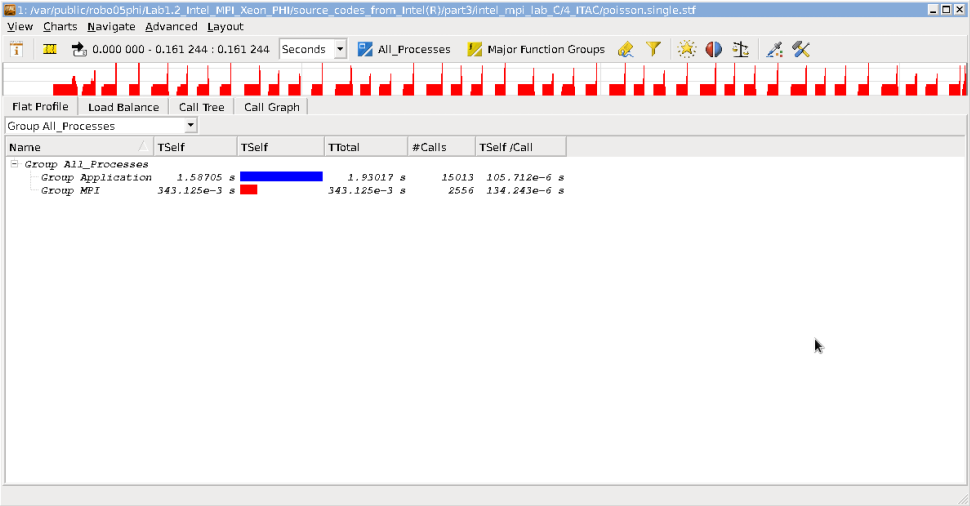
\includegraphics[width=.8\textwidth]{scr1} \\
    \parbox{.8\textwidth}{\center poisson.single.stf \#1} \\[.5em]
    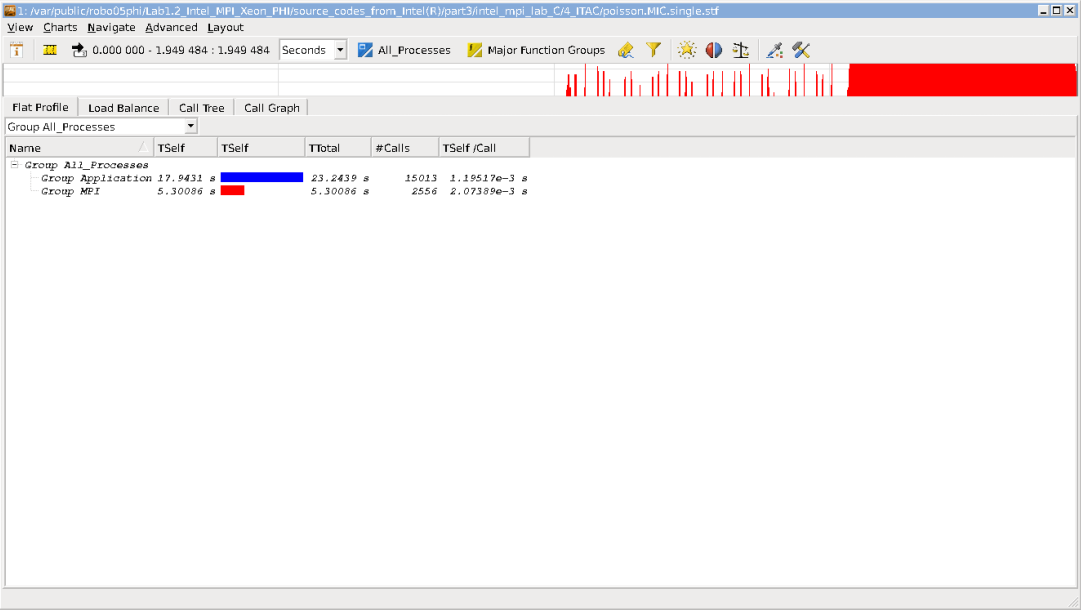
\includegraphics[width=.8\textwidth]{scr2} \\
    \parbox{.8\textwidth}{\center poisson.MIC.single.stf} \\[.5em]
    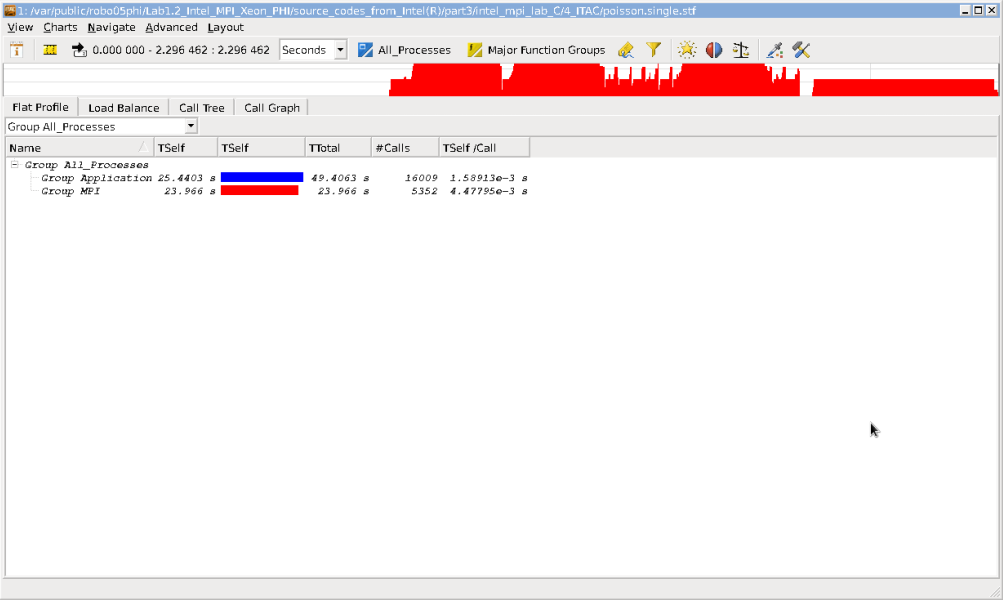
\includegraphics[width=.8\textwidth]{scr3} \\
    \parbox{.8\textwidth}{\center poisson.single.stf \#2}
  \end{figure}

\end{document}
\end{document}
